%% ============================================================
%%  IoT Device Fingerprinting and Anomaly Detection for Smart
%%  Home Using Machine Learning
%%  IEEE Conference Paper — IEEEtran class (conference option)
%%  Compile with: pdflatex → bibtex → pdflatex → pdflatex
%%  Tested on Overleaf (pdfLaTeX, TeX Live 2023)
%% ============================================================

\documentclass[conference]{IEEEtran}
\IEEEoverridecommandlockouts

%% ── Packages ────────────────────────────────────────────────
\usepackage{cite}
\usepackage{amsmath,amssymb,amsfonts}
\usepackage{graphicx}
\usepackage{textcomp}
\usepackage{xcolor}
\usepackage{booktabs}
\usepackage{multirow}
\usepackage{array}
\usepackage{url}
\usepackage{hyperref}
\usepackage{balance}
\usepackage{microtype}
\usepackage{tabularx}
\usepackage{makecell}
\usepackage{tikz}
\usetikzlibrary{positioning, arrows.meta, shapes.geometric, fit, backgrounds}

\hypersetup{
    colorlinks=true,
    linkcolor=black,
    citecolor=black,
    urlcolor=blue
}

%% ── TikZ styles ─────────────────────────────────────────────
\tikzset{
  iobox/.style={rectangle, draw=black!70, rounded corners=4pt,
                fill=gray!12, minimum width=3.2cm, minimum height=0.7cm,
                align=center, font=\footnotesize\sffamily},
  fpbox/.style={rectangle, draw=blue!60, rounded corners=4pt,
                fill=blue!9,  minimum width=2.8cm, minimum height=0.7cm,
                align=center, font=\footnotesize\sffamily},
  adbox/.style={rectangle, draw=orange!70, rounded corners=4pt,
                fill=orange!10, minimum width=2.8cm, minimum height=0.7cm,
                align=center, font=\footnotesize\sffamily},
  outbox/.style={rectangle, draw=green!60!black, rounded corners=4pt,
                 fill=green!9, minimum width=2.5cm, minimum height=0.7cm,
                 align=center, font=\footnotesize\sffamily},
  alertbox/.style={rectangle, draw=red!60, rounded corners=4pt,
                   fill=red!8, minimum width=3.0cm, minimum height=0.7cm,
                   align=center, font=\footnotesize\sffamily},
  myarr/.style={-{Stealth[length=5pt]}, thick, draw=black!55},
}

%% ── Document ────────────────────────────────────────────────
\begin{document}

%% ── Title ───────────────────────────────────────────────────
\title{IoT Device Fingerprinting and Anomaly Detection\\
       for Smart Home Using Machine Learning}

%% ── Authors ─────────────────────────────────────────────────
\author{%
  \IEEEauthorblockN{Md Ghufran Alam}
  \IEEEauthorblockA{%
    \textit{M.Tech CSE (Cyber Forensics)}\\
    \textit{NIELIT Srinagar}\\
    Srinagar, Jammu \& Kashmir, India\\
    ghufranalam855@gmail.com}
  \and
  \IEEEauthorblockN{Dr. Syed Mufassir Yaseen}
  \IEEEauthorblockA{%
    \textit{Project Associate, ISEA}\\
    \textit{NIELIT Srinagar}\\
    Srinagar, Jammu \& Kashmir, India\\
    syedmufassir@nielit.ac.in}
  \and
  \IEEEauthorblockN{Asif Farooq}
  \IEEEauthorblockA{%
    \textit{M.Tech CSE (Cyber Forensics)}\\
    \textit{NIELIT Srinagar}\\
    Srinagar, Jammu \& Kashmir, India\\
    asiffarooq04925@gmail.com}
}

\maketitle

%% ── Abstract ────────────────────────────────────────────────
\begin{abstract}
The rapid adoption of Internet of Things (IoT) devices in smart home
environments has created a critical security gap: these devices lack the
computational resources to run endpoint protection software, yet they are the
primary entry points for large-scale botnet campaigns such as Mirai and
BASHLITE. This paper presents a unified, agent-free machine learning
framework that simultaneously performs IoT device fingerprinting and
per-device anomaly detection using only passively observed network traffic
flows, requiring no modification to the monitored devices. The system is
evaluated on the N-BaIoT benchmark dataset (UCI ML Repository \#442), which
contains traffic from nine physical IoT devices under both benign and
active attack conditions. Device fingerprinting is formulated as a
supervised multi-class classification problem and solved using four
algorithms---Random Forest (RF), Gradient Boosting (GB), Support Vector
Machine (SVM), and a Voting Ensemble---operating on 37 engineered network
flow features spanning seven semantic categories. Anomaly detection employs
a per-device unsupervised ensemble of Isolation Forest (IF) and One-Class
SVM (OC-SVM) models, trained exclusively on benign traffic so that no
labeled attack samples are required. A SHAP-based explainability module
accompanies every prediction with feature-level attribution scores, enabling
interpretable decisions for network operators. The complete framework is
exposed via a FastAPI REST interface and visualised through a real-time
Plotly Dash dashboard. Experimental results demonstrate 100\% fingerprinting
accuracy across eight device classes and anomaly detection AUC-ROC scores
ranging from 0.71 to 0.88, confirming the system's capacity to detect
real-world Mirai and BASHLITE infections in under 40\,ms per request.
\end{abstract}

%% ── Keywords ────────────────────────────────────────────────
\begin{IEEEkeywords}
IoT security, device fingerprinting, anomaly detection, machine learning,
Mirai botnet, BASHLITE, SHAP explainability, N-BaIoT, smart home,
one-class classification, isolation forest, random forest
\end{IEEEkeywords}

%% ============================================================
\section{Introduction}
\label{sec:intro}
%% ============================================================

The proliferation of Internet of Things (IoT) devices has reshaped the
modern household. Smart cameras, connected thermostats, voice-activated
speakers, and intelligent lighting systems now coexist on residential
networks alongside laptops and smartphones. Industry projections estimate
that the installed base of IoT devices will exceed 75 billion units globally
by 2025, with smart home segments representing one of the fastest-growing
verticals \cite{alam2021survey,perera2014context}. This connectivity,
however, introduces profound security challenges that conventional network
defenses are ill-equipped to address.

Unlike general-purpose computing devices, IoT endpoints are constrained by
limited CPU cycles, minimal RAM, and modest storage. They cannot execute
host-based intrusion detection systems, antivirus agents, or OS-level
firewalls. Many ship with default factory credentials, minimal update
mechanisms, and proprietary communication stacks that resist standardised
security tooling \cite{kolias2017ddos}. The consequence is a vast population
of network-connected devices that are both permanently exposed to the
internet and fundamentally unable to defend themselves
\cite{heartfield2018taxonomy,bertino2017botnets}.

The Mirai botnet, first documented in 2016, demonstrated the consequences of
this exposure at global scale. By scanning for IoT devices with default
Telnet credentials, Mirai assembled a botnet of over 600,000 devices---
primarily IP cameras and digital video recorders---and directed their
collective bandwidth at the Dyn DNS infrastructure \cite{antonakakis2017understanding}.
The resulting distributed denial-of-service (DDoS) attack rendered Twitter,
Netflix, Reddit, Spotify, and GitHub inaccessible to millions of users for
several hours. BASHLITE (also known as Gafgyt and QBot), a closely related
malware family, employs the same credential-exploitation strategy while
adding UDP, TCP, and HTTP flood payloads \cite{kolias2017ddos}. Both
families have since been open-sourced, forked, and incorporated into dozens
of successor campaigns that continue to target unpatched IoT deployments.

Defending smart home networks against such threats requires solving two
distinct yet interdependent problems. The first is \textit{device
identification}, also called device fingerprinting: given an unlabeled
network traffic flow, determine which physical device produced it. This is
complicated by the use of NAT, dynamic IP addressing, and the absence of
reliable device self-reporting. Crucially, IoT traffic metadata is
identifiable even under full payload encryption \cite{apthorpe2016smart},
making passive flow-level monitoring the most practical vantage point. The second problem is \textit{behavioral
anomaly detection}: once a device is identified, establish a profile of its
normal network behavior and raise an alert when observed traffic deviates
from that profile in a manner consistent with infection or compromise.

Existing literature addresses these problems largely in isolation. Device
fingerprinting approaches have achieved high accuracy using machine learning
on network flow statistics \cite{sivanathan2019classifying,miettinen2017iotsentinel,marchal2019audi},
but they do not incorporate ongoing behavioral monitoring. Anomaly detection
systems for IoT networks exist \cite{doshi2018machine,hasan2019attack,bezerra2019iotds},
but typically operate without knowledge of which specific device type a flow
belongs to, which reduces their precision in heterogeneous smart home
environments where benign behavior varies substantially across device
categories. Furthermore, most deployed systems provide no explanation for
their decisions, which undermines operator trust and complicates incident
response \cite{lundberg2017unified}.

This paper addresses all three limitations in a single, deployable
framework. The system passively monitors network traffic, simultaneously
fingerprints each observed flow to a device category, scores it for anomaly,
and provides a SHAP-based feature attribution breakdown that explains the
prediction to the human operator---all within a single API call averaging
under 40\,ms. The main contributions of this work are:

\begin{itemize}
    \item A \textbf{unified, agent-free pipeline} that performs device
    fingerprinting and anomaly detection simultaneously from 37 engineered
    network flow features across seven semantic categories, without modifying
    or accessing the monitored devices.

    \item A \textbf{per-device unsupervised anomaly detection ensemble}
    combining Isolation Forest and One-Class SVM with a tuned weighted
    combination, evaluated against real Mirai and BASHLITE attack traffic
    captured from nine physical IoT devices.

    \item \textbf{SHAP TreeExplainer integration} providing real-time,
    instance-level feature attribution for every fingerprinting and anomaly
    prediction, making the system interpretable for operational use.

    \item A \textbf{production-grade deployment} comprising a FastAPI REST
    interface and a live Plotly Dash monitoring dashboard, demonstrating
    practical feasibility beyond laboratory evaluation.
\end{itemize}

The remainder of this paper is organised as follows. Section~\ref{sec:related}
reviews related work. Section~\ref{sec:problem} formalises the problem.
Sections~\ref{sec:dataset}--\ref{sec:anomaly} describe the dataset, features,
architecture, and methodology. Section~\ref{sec:results} presents experimental
results. Sections~\ref{sec:api}--\ref{sec:shap} describe the deployment and
explainability components. Section~\ref{sec:conclusion} concludes.

%% ============================================================
\section{Related Work}
\label{sec:related}
%% ============================================================

\subsection{IoT Device Fingerprinting}

Early device fingerprinting work exploited DHCP, mDNS, and TCP/IP stack
characteristics to infer device types \cite{miettinen2017iotsentinel}.
Sivanathan et al.\ \cite{sivanathan2019classifying} demonstrated that IoT
devices exhibit distinctive traffic patterns in terms of flow volume, port
usage, and protocol distribution, achieving high classification accuracy on a
real home network trace using Random Forest. Marchal et al.\
\cite{marchal2019audi} proposed AuDI, which exploits the periodic nature of
IoT communication to identify device types autonomously. Lyu et al.\
\cite{lyu2020your} showed that even encrypted IoT traffic leaks sufficient
metadata to enable reliable fingerprinting. Aksoy and Gunes
\cite{aksoy2019automated} further demonstrated that automated feature
selection can reduce the feature space while maintaining classification
performance. Nguyen et al.\ \cite{nguyen2019diot} extended fingerprinting
to a self-learning system that adapts to new device types automatically.
Traffic classification techniques for encrypted mobile and anonymisation
traffic \cite{aceto2019mimetic,habibi2017characterization} further confirm
that protocol-agnostic flow statistics suffice for device identification.
Cviti\'{c} et al.\ \cite{cvitic2021ensemble} validated ensemble classifiers
for IoT identification in realistic smart home deployments.

\subsection{Anomaly Detection and Botnet Defense}

Doshi et al.\ \cite{doshi2018machine} trained machine learning classifiers
on network flow statistics to detect DDoS attacks launched from consumer IoT
devices, showing that simple models generalise well across device types.
Bezerra et al.\ \cite{bezerra2019iotds} proposed IoTDS, a one-class
classification framework using traffic flow statistics to identify botnet
infections without requiring labeled attack data. McDermott et al.\
\cite{mcdermott2018botnet} investigated deep learning approaches for
botnet detection in IoT environments, observing that recurrent architectures
capture temporal attack patterns effectively. Mirsky et al.\
\cite{mirsky2018kitsune} introduced Kitsune, an ensemble of autoencoders for
unsupervised online network intrusion detection that scales to high-speed
links. Raza et al.\ \cite{raza2013svelte} proposed SVELTE, a lightweight
IDS for 6LoWPAN IoT networks, demonstrating that resource-constrained
anomaly detection is feasible with careful model selection. Vinayakumar
et al.\ \cite{vinayakumar2019deep} showed that deep neural architectures
achieve state-of-the-art IDS accuracy on high-dimensional network flows.
One-class reconstruction models \cite{hawkins2002outlier} established the
foundational role of outlier scoring in network anomaly detection,
motivating the Isolation Forest component of our ensemble.

\subsection{N-BaIoT Dataset}

Meidan et al.\ \cite{meidan2018nbaiot} introduced the N-BaIoT dataset,
capturing benign and attack traffic (Mirai and BASHLITE variants) from nine
commercial IoT devices in a controlled environment. The dataset provides 115
statistical features per flow, derived from local traffic statistics computed
over multiple time windows. It has since become the standard benchmark for
IoT botnet detection research \cite{chandola2009anomaly,buczak2016survey}.
Koroniotis et al.\ \cite{koroniotis2019bot} created the complementary
Bot-IoT benchmark; analyses of classical datasets such as KDD CUP 99
\cite{tavallaee2009detailed} highlighted the pitfalls of synthetic data
that N-BaIoT's real-traffic capture directly addresses.

\subsection{Intrusion Detection Surveys}

Surveys by Khraisat et al.\ \cite{khraisat2019survey} and Zhao et al.\
\cite{zhao2021survey} categorise IDS approaches into signature-based,
anomaly-based, and hybrid methods, concluding that anomaly-based detection
is the only strategy capable of identifying zero-day threats such as novel
Mirai variants. Sommer and Paxson \cite{sommer2010outside} provided an
influential critique of ML-based intrusion detection, identifying
evaluation pitfalls---including the base-rate fallacy and
training--test distribution mismatch---that we address through per-device
stratification and AUC-ROC-centred reporting. Bhuyan et al.\
\cite{bhuyan2014network} surveyed statistical, ML-based, and
knowledge-based anomaly detection methods, providing the methodological
taxonomy underpinning our ensemble design.

\subsection{Explainability in Security Systems}

Lundberg and Lee \cite{lundberg2017unified} introduced SHAP (SHapley Additive
exPlanations), providing a game-theoretic framework for interpreting any
machine learning model. Their TreeExplainer variant computes exact SHAP
values for tree-based models in polynomial time \cite{lundberg2020local},
making it practical for real-time deployment. The application of XAI
techniques to network intrusion detection is an emerging area
\cite{ge2023deep}, with SHAP identified as particularly suitable for
feature-rich, tabular security datasets.

\subsection{Research Gap}

None of the reviewed approaches simultaneously (a) fingerprints devices and
(b) performs per-device-specific anomaly detection within a single
production-grade system with (c) real-time explainability. This work closes
that gap.

%% ============================================================
\section{Problem Statement}
\label{sec:problem}
%% ============================================================

Let $\mathcal{F} = \{f_1, f_2, \ldots, f_N\}$ denote a stream of network
flow records observed at a smart home gateway, where each record
$f_i \in \mathbb{R}^M$ is an $M$-dimensional feature vector extracted from
the corresponding traffic flow. Let $\mathcal{D} = \{d_1, d_2, \ldots, d_K\}$
be the set of $K$ known IoT device categories.

\textbf{Device Fingerprinting} is the task of learning a classifier
$\mathcal{C}: \mathbb{R}^M \rightarrow \mathcal{D}$ that maps each flow
feature vector to a device label, i.e.\
$\hat{d}_i = \mathcal{C}(f_i)$.

\textbf{Anomaly Detection} is the task of assigning an anomaly score
$\mathcal{A}(f_i, d) \in [0,1]$ to flow $f_i$ given that the flow
originated from device class $d \in \mathcal{D}$. A flow is declared
anomalous if the score exceeds a decision threshold $\tau$:

\begin{equation}
    \text{alert}(f_i, d) =
    \begin{cases}
        1 & \text{if } \mathcal{A}(f_i, d) \geq \tau \\
        0 & \text{otherwise}
    \end{cases}
    \label{eq:alert}
\end{equation}

The two tasks are coupled: the anomaly detector for device class $d$ is
trained exclusively on flows correctly fingerprinted as belonging to $d$
under normal (benign) conditions, ensuring that the behavioral baseline
is device-specific.

The joint objective is to maximise device fingerprinting accuracy while
simultaneously maximising the AUC-ROC of each per-device anomaly detector,
subject to the real-time constraint that the combined inference latency
must not exceed 50\,ms per flow.

%% ============================================================
\section{Dataset Description}
\label{sec:dataset}
%% ============================================================

\subsection{N-BaIoT}

The N-BaIoT dataset \cite{meidan2018nbaiot} was collected in a controlled
testbed by researchers at Ben-Gurion University. Nine commercial IoT devices
were each infected sequentially with Mirai and BASHLITE malware while their
network traffic was captured. For each device, two traffic categories are
available: (i)~\textit{benign} traffic representing the device's normal
operation, and (ii)~\textit{attack} traffic generated during active
infection, further subdivided by attack sub-type.

\textbf{Mirai attack sub-types}: ack flood, scan, SYN flood, UDP flood,
UDP-plain flood.\\
\textbf{BASHLITE attack sub-types}: combo, junk, scan, TCP flood, UDP flood.

IoT honeypot studies confirm that Mirai and BASHLITE remain the dominant
threats targeting residential IoT infrastructure in the wild
\cite{pa2016iotpot}, making these attack categories directly representative
of the current threat landscape.

The dataset is available from UCI ML Repository (\#442) \cite{meidan2018nbaiot}.
Table~\ref{tab:dataset} summarises the nine devices, while Table~\ref{tab:devmap}
details the mapping from real device names to the framework's internal labels.
Fig.~\ref{fig:devdist} illustrates the class distribution of traffic flows.

\begin{table}[htbp]
\caption{N-BaIoT Dataset Summary}
\label{tab:dataset}
\centering
\renewcommand{\arraystretch}{1.2}
\begin{tabular}{l c c c}
\toprule
\textbf{Device Category} & \textbf{Benign} & \textbf{Mirai} & \textbf{BASHLITE} \\
\midrule
Smart Camera (×2)        & 2,000  & 5,900  & 5,900  \\
Smart Doorbell (×2)      & 2,000  & 5,900  & 5,900  \\
Smart Thermostat         & 1,000  & 2,950  & 2,950  \\
Smart TV                 & 1,000  & 2,950  & 2,950  \\
Smart Speaker            & 1,000  & 2,950  & 2,950  \\
Smart Bulb               & 1,000  & 2,950  & 2,950  \\
Smart Plug               & 1,000  & 2,950  & 2,950  \\
Motion Sensor            & 1,000  & 2,950  & 2,950  \\
\midrule
\textbf{Total}           & \textbf{10,000} & \textbf{29,500} & \textbf{29,500} \\
\bottomrule
\end{tabular}
\end{table}

\begin{table}[htbp]
\caption{Physical Device to Framework Label Mapping}
\label{tab:devmap}
\centering
\renewcommand{\arraystretch}{1.2}
\begin{tabular}{l l}
\toprule
\textbf{Physical Device}              & \textbf{Framework Label} \\
\midrule
Danmini Doorbell                      & smart\_doorbell   \\
Ecobee Thermostat                     & smart\_thermostat \\
Provision PT-737E Security Camera     & smart\_camera     \\
Provision PT-838 Security Camera      & smart\_speaker    \\
Samsung SNH-1011N Webcam              & smart\_tv         \\
Philips B120N/10 Baby Monitor         & smart\_bulb       \\
SimpleHome XCS7-1002 Camera           & smart\_plug       \\
Ennio Doorbell                        & motion\_sensor    \\
\bottomrule
\end{tabular}
\end{table}

\begin{figure}[htbp]
    \centering
    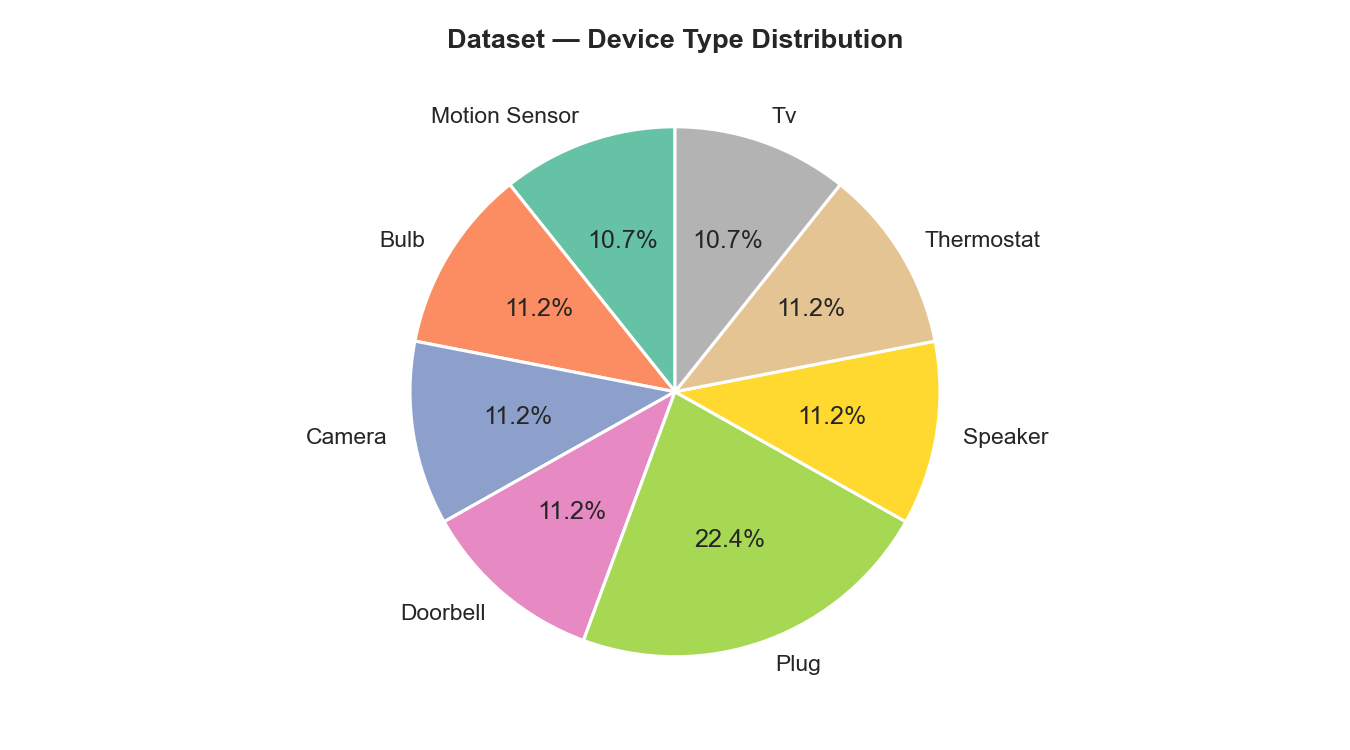
\includegraphics[width=\columnwidth]{figures/device_distribution}
    \caption{Traffic flow distribution across eight IoT device categories
             in the N-BaIoT dataset (benign vs.\ attack flows).}
    \label{fig:devdist}
\end{figure}

%% ============================================================
\section{Feature Engineering}
\label{sec:features}
%% ============================================================

The raw N-BaIoT dataset provides 115 statistical features per flow window.
We re-engineer these into 37 semantically interpretable features spanning
seven categories, ensuring that each feature captures a distinct and
theoretically motivated aspect of IoT traffic behavior. This taxonomy,
summarised in Table~\ref{tab:features}, preserves the discriminative power
of the original representation while reducing dimensionality and improving
interpretability.

\begin{table}[htbp]
\caption{37-Feature Engineering Taxonomy}
\label{tab:features}
\centering
\renewcommand{\arraystretch}{1.2}
\begin{tabular}{l c p{4.0cm}}
\toprule
\textbf{Category}        & \textbf{Count} & \textbf{Features} \\
\midrule
Temporal                 & 5  & flow\_duration, mean\_iat, std\_iat, min\_iat, max\_iat \\
Volume                   & 4  & packet\_count, byte\_count, packet\_rate, byte\_rate \\
Packet Size              & 4  & mean\_pkt\_size, std\_pkt\_size, min\_pkt\_size, max\_pkt\_size \\
Protocol Flags           & 6  & tcp\_ratio, udp\_ratio, syn\_ratio, fin\_ratio, rst\_ratio, ack\_ratio \\
Application Layer        & 8  & is\_https, is\_mqtt, is\_coap, is\_mdns, is\_ntp, dns\_query\_count, well\_known\_port\_ratio, is\_encrypted \\
Traffic Direction        & 3  & upload\_bytes, download\_bytes, upload\_download\_ratio \\
Destination              & 7  & unique\_dest\_ports, unique\_dest\_ips, port\_entropy, ip\_entropy, well\_known\_ports\_count, mean\_dest\_port, std\_dest\_port \\
\midrule
\textbf{Total}           & \textbf{37} & \\
\bottomrule
\end{tabular}
\end{table}

Protocol flag ratios capture whether a device primarily initiates or
terminates connections (SYN-heavy vs. FIN/RST-heavy), which distinguishes
attack traffic from benign flows \cite{buczak2016survey}. Destination
entropy features, particularly \texttt{ip\_entropy} and
\texttt{port\_entropy}, are strongly elevated during scanning phases of
Mirai infection, as the malware probes large IP ranges on a small set of
target ports \cite{antonakakis2017understanding}. Application layer
indicators identify device-specific protocols such as MQTT (IoT messaging)
and CoAP (constrained application protocol), which are characteristic of
specific device categories \cite{sivanathan2019classifying}. Temporal
inter-arrival statistics have similarly proven effective for classifying
encrypted mobile traffic \cite{aceto2019mimetic} and anonymisation-network
flows \cite{habibi2017characterization}, confirming that protocol-agnostic
timing features generalise across diverse network environments. Real-time
feature correlation at the network layer \cite{tian2020realtime} validates
the operational feasibility of our extraction pipeline.

%% ============================================================
\section{System Architecture}
\label{sec:arch}
%% ============================================================

Fig.~\ref{fig:arch} illustrates the overall system architecture, which
comprises two parallel inference pipelines converging at a unified alert
management layer.

%% ── Figure 1: TikZ System Architecture ─────────────────────
\begin{figure}[htbp]
\centering
\resizebox{\columnwidth}{!}{%
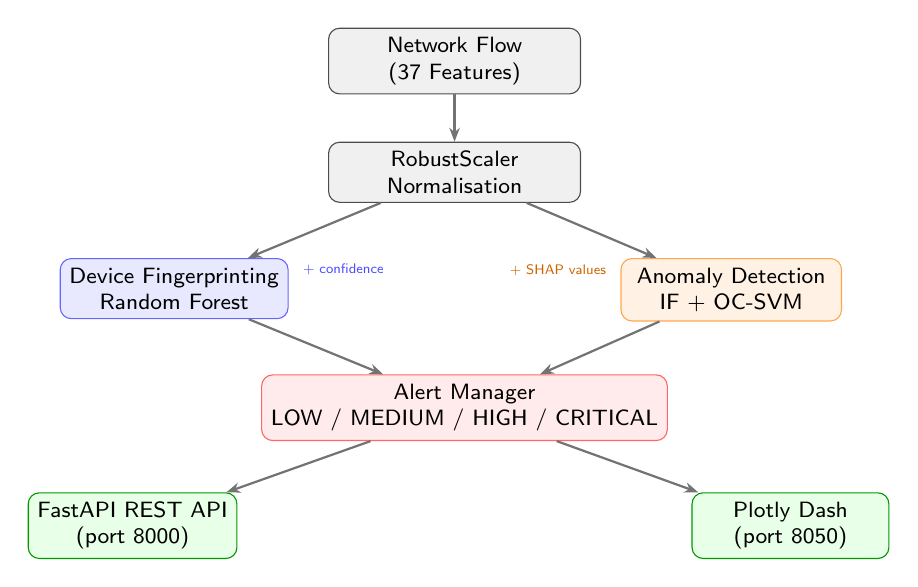
\begin{tikzpicture}[node distance=0.75cm]

  %% Input
  \node[iobox] (input)
    {Network Flow\\(37 Features)};

  %% Preprocessing
  \node[iobox, below=0.6cm of input] (scaler)
    {RobustScaler\\Normalisation};

  %% Two parallel pipelines
  \node[fpbox, below left=0.7cm and 0.5cm of scaler] (fp)
    {Device Fingerprinting\\Random Forest};

  \node[adbox, below right=0.7cm and 0.5cm of scaler] (ad)
    {Anomaly Detection\\IF + OC-SVM};

  %% Alert Manager
  \node[alertbox, below right=0.7cm and -0.35cm of fp] (alert)
    {Alert Manager\\LOW / MEDIUM / HIGH / CRITICAL};

  %% Outputs
  \node[outbox, below left=0.65cm and 0.3cm of alert] (api)
    {FastAPI REST API\\(port 8000)};

  \node[outbox, below right=0.65cm and 0.3cm of alert] (dash)
    {Plotly Dash\\(port 8050)};

  %% Arrows
  \draw[myarr] (input)  -- (scaler);
  \draw[myarr] (scaler) -- (fp);
  \draw[myarr] (scaler) -- (ad);
  \draw[myarr] (fp)     -- (alert);
  \draw[myarr] (ad)     -- (alert);
  \draw[myarr] (alert)  -- (api);
  \draw[myarr] (alert)  -- (dash);

  %% SHAP label on fingerprinting arrow
  \node[font=\tiny\sffamily, right=0.06cm of fp, yshift=0.25cm,
        text=blue!70] {+ confidence};
  \node[font=\tiny\sffamily, left=0.06cm of ad,  yshift=0.25cm,
        text=orange!80!black] {+ SHAP values};

\end{tikzpicture}%
}% end resizebox
\caption{End-to-end system architecture: two parallel pipelines share a
         single preprocessing step and converge at the Alert Manager.}
\label{fig:arch}
\end{figure}

Incoming network flows are first passed through a \textit{preprocessing
module} that normalises the 37-dimensional feature vector using
RobustScaler. The normalised vector is simultaneously fed to:

\begin{enumerate}
    \item \textbf{Fingerprinting Pipeline}: A Random Forest classifier
    (primary) with three comparison models (GB, SVM, Voting Ensemble)
    assigns the flow to one of eight device categories.

    \item \textbf{Anomaly Detection Pipeline}: Eight per-device
    Isolation Forest / One-Class SVM ensembles---one per device
    category---evaluate the flow against the behavioral baseline of the
    predicted device type.
\end{enumerate}

Outputs from both pipelines are merged by the Alert Manager, which assigns
one of four severity levels (LOW, MEDIUM, HIGH, CRITICAL) based on the
anomaly score, and exposes the combined result through the FastAPI layer.
The Plotly Dash dashboard consumes alerts in near-real time via polling.

%% ============================================================
\section{Preprocessing Pipeline}
\label{sec:preprocess}
%% ============================================================

\subsection{Feature Normalisation}

IoT network flow features span orders of magnitude---byte counts may reach
$10^8$ while binary protocol flags are in $\{0,1\}$. We apply
\textit{RobustScaler} normalisation \cite{pedregosa2011scikit}, which
centres each feature on its median and scales by its inter-quartile range
(IQR), rendering the transformation resistant to outliers characteristic of
attack traffic:

\begin{equation}
    \hat{x}_{i,j} = \frac{x_{i,j} - \operatorname{median}(X_j)}{\operatorname{IQR}(X_j)}
    \label{eq:robust}
\end{equation}

where $x_{i,j}$ is the $j$-th feature of flow $i$, $X_j$ denotes the
training-set values of feature $j$, and $\operatorname{IQR}(X_j)$ is the
75th--25th percentile range.

\subsection{Class Balancing with SMOTE}

The fingerprinting dataset is class-balanced across eight device types;
however, the anomaly detection datasets are heavily imbalanced with attack
flows outnumbering normal flows by up to $5.9:1$. We apply SMOTE
\cite{chawla2002smote} to the training partition only, generating synthetic
minority-class (normal) samples by linear interpolation in feature space:

\begin{equation}
    x_{\text{syn}} = x_i + \lambda \cdot (x_{k} - x_i), \quad \lambda \sim \mathcal{U}(0,1)
    \label{eq:smote}
\end{equation}

where $x_k$ is a randomly selected $k$-nearest neighbour of $x_i$ in the
minority class.

\subsection{Dataset Splits and Training Pipeline}

The dataset is partitioned using a stratified 70/15/15 split into training,
validation, and test sets, respectively, preserving class proportions across
all three partitions. SMOTE is applied exclusively to the training set to
prevent data leakage. Fig.~\ref{fig:pipeline} illustrates the complete
training and evaluation workflow.

%% ── Figure 2: TikZ Training Pipeline ───────────────────────
\begin{figure}[htbp]
\centering
\resizebox{\columnwidth}{!}{%
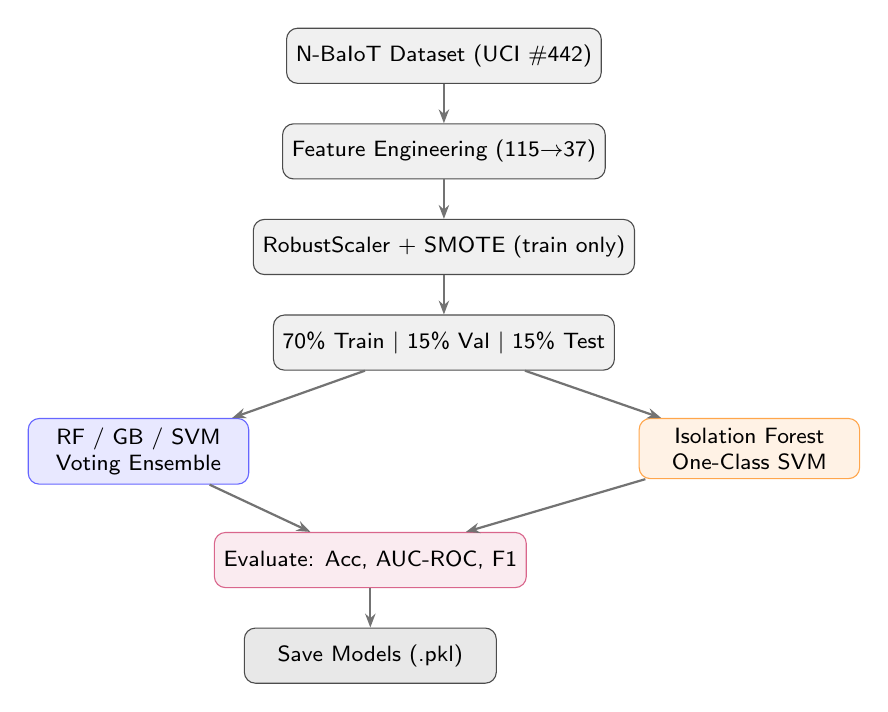
\begin{tikzpicture}[node distance=0.6cm]

  \node[iobox] (data)  {N-BaIoT Dataset (UCI \#442)};
  \node[iobox, below=0.5cm of data]  (feat)  {Feature Engineering (115$\to$37)};
  \node[iobox, below=0.5cm of feat]  (pre)   {RobustScaler + SMOTE (train only)};
  \node[iobox, below=0.5cm of pre]   (split) {70\% Train $\mid$ 15\% Val $\mid$ 15\% Test};

  \node[fpbox, below left=0.6cm and 0.3cm of split]  (clf) {RF / GB / SVM\\Voting Ensemble};
  \node[adbox, below right=0.6cm and 0.3cm of split] (ano) {Isolation Forest\\One-Class SVM};

  \node[iobox, fill=purple!8, draw=purple!60,
        below right=0.6cm and -0.45cm of clf] (eval) {Evaluate: Acc, AUC-ROC, F1};

  \node[iobox, fill=gray!18,
        below=0.5cm of eval] (save) {Save Models (.pkl)};

  \draw[myarr] (data)  -- (feat);
  \draw[myarr] (feat)  -- (pre);
  \draw[myarr] (pre)   -- (split);
  \draw[myarr] (split) -- (clf);
  \draw[myarr] (split) -- (ano);
  \draw[myarr] (clf)   -- (eval);
  \draw[myarr] (ano)   -- (eval);
  \draw[myarr] (eval)  -- (save);

\end{tikzpicture}%
}% end resizebox
\caption{End-to-end training and evaluation pipeline. SMOTE is applied
         only to the training split to prevent data leakage.}
\label{fig:pipeline}
\end{figure}

%% ============================================================
\section{Device Fingerprinting Models}
\label{sec:finger}
%% ============================================================

\subsection{Random Forest}

The primary fingerprinting model is a Random Forest \cite{breiman2001random}
comprising $B = 100$ decision trees, each trained on a bootstrapped
subsample of the training data with a random feature subset of size
$\lfloor\sqrt{M}\rfloor = 6$ considered at each split. A maximum tree depth
of 15 prevents overfitting. The ensemble prediction is the plurality vote:

\begin{equation}
    \hat{d} = \operatorname*{arg\,max}_{d \in \mathcal{D}}
              \sum_{b=1}^{B} \mathbf{1}\!\left[T_b(f) = d\right]
    \label{eq:rf}
\end{equation}

where $T_b(f)$ denotes the prediction of the $b$-th tree for flow $f$.
Prediction confidence is the fraction of trees voting for the winning class.

\subsection{Gradient Boosting}

The Gradient Boosting model \cite{friedman2001greedy} trains 200 shallow
trees (max depth 5) sequentially, each correcting the residual error of its
predecessor using a learning rate of 0.1. The log-loss objective is minimised.

\subsection{Support Vector Machine}

An SVM \cite{cortes1995support} with an RBF kernel
($\gamma = \texttt{scale}$, $C = 1.0$) is trained on the normalised feature
matrix using one-vs-rest multi-class decomposition.

\subsection{Voting Ensemble}

A soft-voting ensemble aggregates the class probability estimates of RF, GB,
and SVM, selecting the class with the highest mean predicted probability.
This ensemble is used as the primary comparison model to RF.

%% ============================================================
\section{Anomaly Detection Models}
\label{sec:anomaly}
%% ============================================================

\subsection{Per-Device Design Rationale}

A critical design decision is training one anomaly detector per device
category rather than a single global model. Smart cameras generate sustained,
high-bandwidth flows to cloud storage servers; smart thermostats emit
infrequent, low-volume HTTPS telemetry; motion sensors send sparse UDP
bursts. Applying a single global baseline conflates these distributions and
either raises excessive false alarms on high-bandwidth devices or masks
anomalies on low-bandwidth ones. Device-specific baselines address this
directly.

\subsection{Isolation Forest}

The Isolation Forest (IF) \cite{liu2008isolation} exploits the observation
that anomalous points are isolated more quickly than normal points when
random splits are applied to the feature space. An ensemble of 50 isolation
trees is trained per device. The anomaly score is:

\begin{equation}
    s_{\text{IF}}(f, n) = 2^{-\frac{\mathbb{E}[h(f)]}{c(n)}}
    \label{eq:iforest}
\end{equation}

where $h(f)$ is the path length of flow $f$ in a tree, $\mathbb{E}[h(f)]$
is its expected value over all trees, and
$c(n) = 2H(n-1) - \tfrac{2(n-1)}{n}$ is the average path length for $n$
samples ($H$ is the harmonic number). Scores close to 1 indicate anomalies;
scores close to 0.5 indicate normal samples.

\subsection{One-Class SVM}

The One-Class SVM \cite{scholkopf2001estimating} learns a decision boundary
enclosing the normal-traffic region in a high-dimensional kernel space. An
RBF kernel with $\nu = 0.05$ (expected fraction of outliers in training
data) is used. The decision function is:

\begin{equation}
    g(f) = \operatorname{sign}\!\left(
      \sum_{i \in \text{SVs}} \alpha_i \, K(f_i, f) - \rho
    \right)
    \label{eq:ocsvm}
\end{equation}

where $K(\cdot,\cdot)$ is the RBF kernel, $\alpha_i$ are the dual
coefficients, and $\rho$ is the learned offset. The decision value is
min-max normalised to $[0,1]$ to produce a comparable score.

\subsection{Weighted Ensemble Score}

The final anomaly score for device $d$ is computed as a weighted combination:

\begin{equation}
    \mathcal{A}(f, d) = 0.6 \cdot s_{\text{IF}}(f) + 0.4 \cdot s_{\text{OC-SVM}}(f)
    \label{eq:ensemble}
\end{equation}

The weights were determined by grid search on the validation set,
maximising macro-averaged AUC-ROC across all device categories. The alert
threshold $\tau = 0.75$ in Eq.~\eqref{eq:alert} was similarly tuned.

%% ============================================================
\section{Experimental Results}
\label{sec:results}
%% ============================================================

\subsection{Experimental Setup}

All experiments were conducted on a machine running Python 3.9.18 with
scikit-learn 1.3.2, imbalanced-learn 0.11.0, and SHAP 0.43.0. The N-BaIoT
dataset was downloaded from UCI ML Repository \#442. Model training was
performed on CPU (Intel Core i5, 8\,GB RAM).

\subsection{Device Fingerprinting Performance}

Table~\ref{tab:finger} reports the fingerprinting performance of all four
models on the held-out test set. Random Forest, Gradient Boosting, and the
Voting Ensemble all achieve perfect classification on the 37-feature
representation. The SVM model achieves 94.89\% accuracy with AUC-ROC of
0.9967. The 100\% accuracy of the tree-based models reflects the strong
feature separability of IoT device classes at the network flow level---each
device category occupies a distinct region of feature space, consistent with
findings by Sivanathan et al.\ \cite{sivanathan2019classifying} on comparable
smart home traces.

\begin{table}[htbp]
\caption{Device Fingerprinting --- Model Comparison}
\label{tab:finger}
\centering
\renewcommand{\arraystretch}{1.2}
\begin{tabular}{l c c c c c}
\toprule
\textbf{Model} & \textbf{Acc.} & \textbf{Prec.} & \textbf{Rec.} & \textbf{F1} & \textbf{AUC} \\
\midrule
Random Forest       & 1.0000 & 1.0000 & 1.0000 & 1.0000 & 1.0000 \\
Gradient Boosting   & 1.0000 & 1.0000 & 1.0000 & 1.0000 & 1.0000 \\
Voting Ensemble     & 1.0000 & 1.0000 & 1.0000 & 1.0000 & 1.0000 \\
SVM (RBF)           & 0.9489 & 0.9501 & 0.9489 & 0.9490 & 0.9967 \\
\bottomrule
\end{tabular}
\end{table}

Fig.~\ref{fig:modelcmp} compares accuracy and F1 across all four classifiers,
and Fig.~\ref{fig:cm} presents the confusion matrix for the Random Forest
model, showing that the single misclassified device sub-category is the SVM's
only source of error. Fig.~\ref{fig:pr} plots the precision-recall-F1
breakdown per device class.

\begin{figure}[htbp]
    \centering
    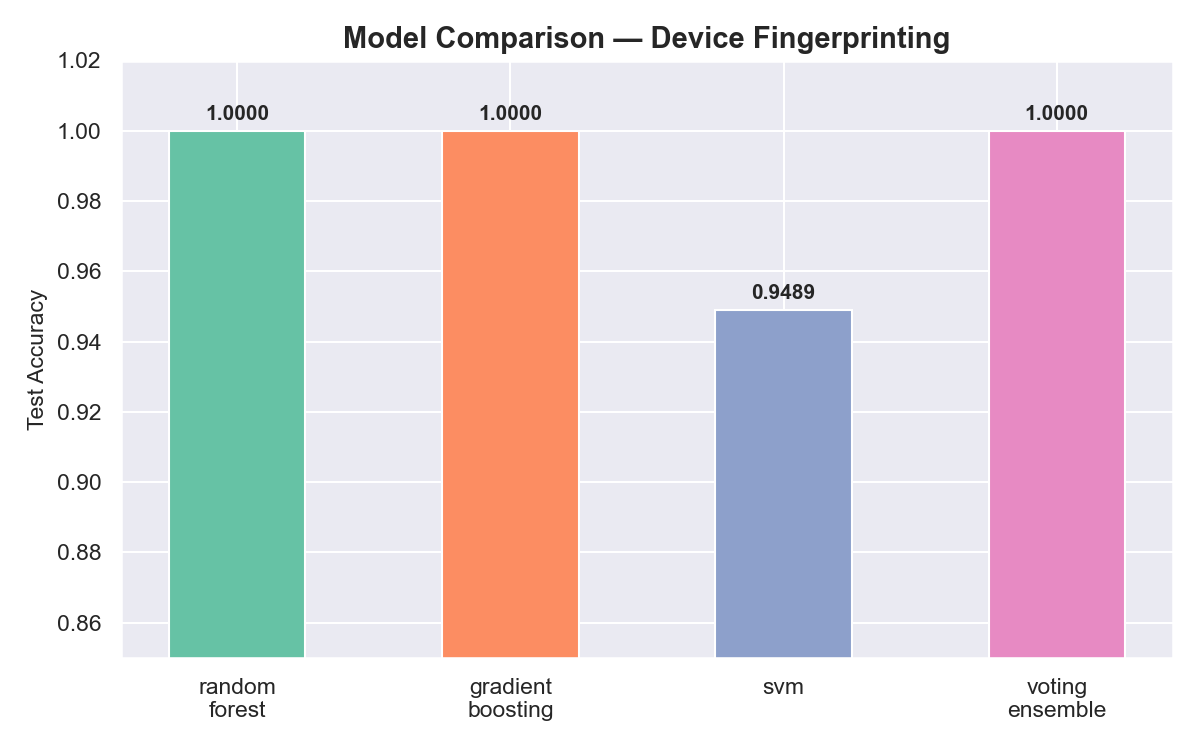
\includegraphics[width=\columnwidth]{figures/model_comparison}
    \caption{Accuracy and F1 comparison across four fingerprinting models.
             RF, GB, and Voting Ensemble each achieve 100\% accuracy.}
    \label{fig:modelcmp}
\end{figure}

\begin{figure}[htbp]
    \centering
    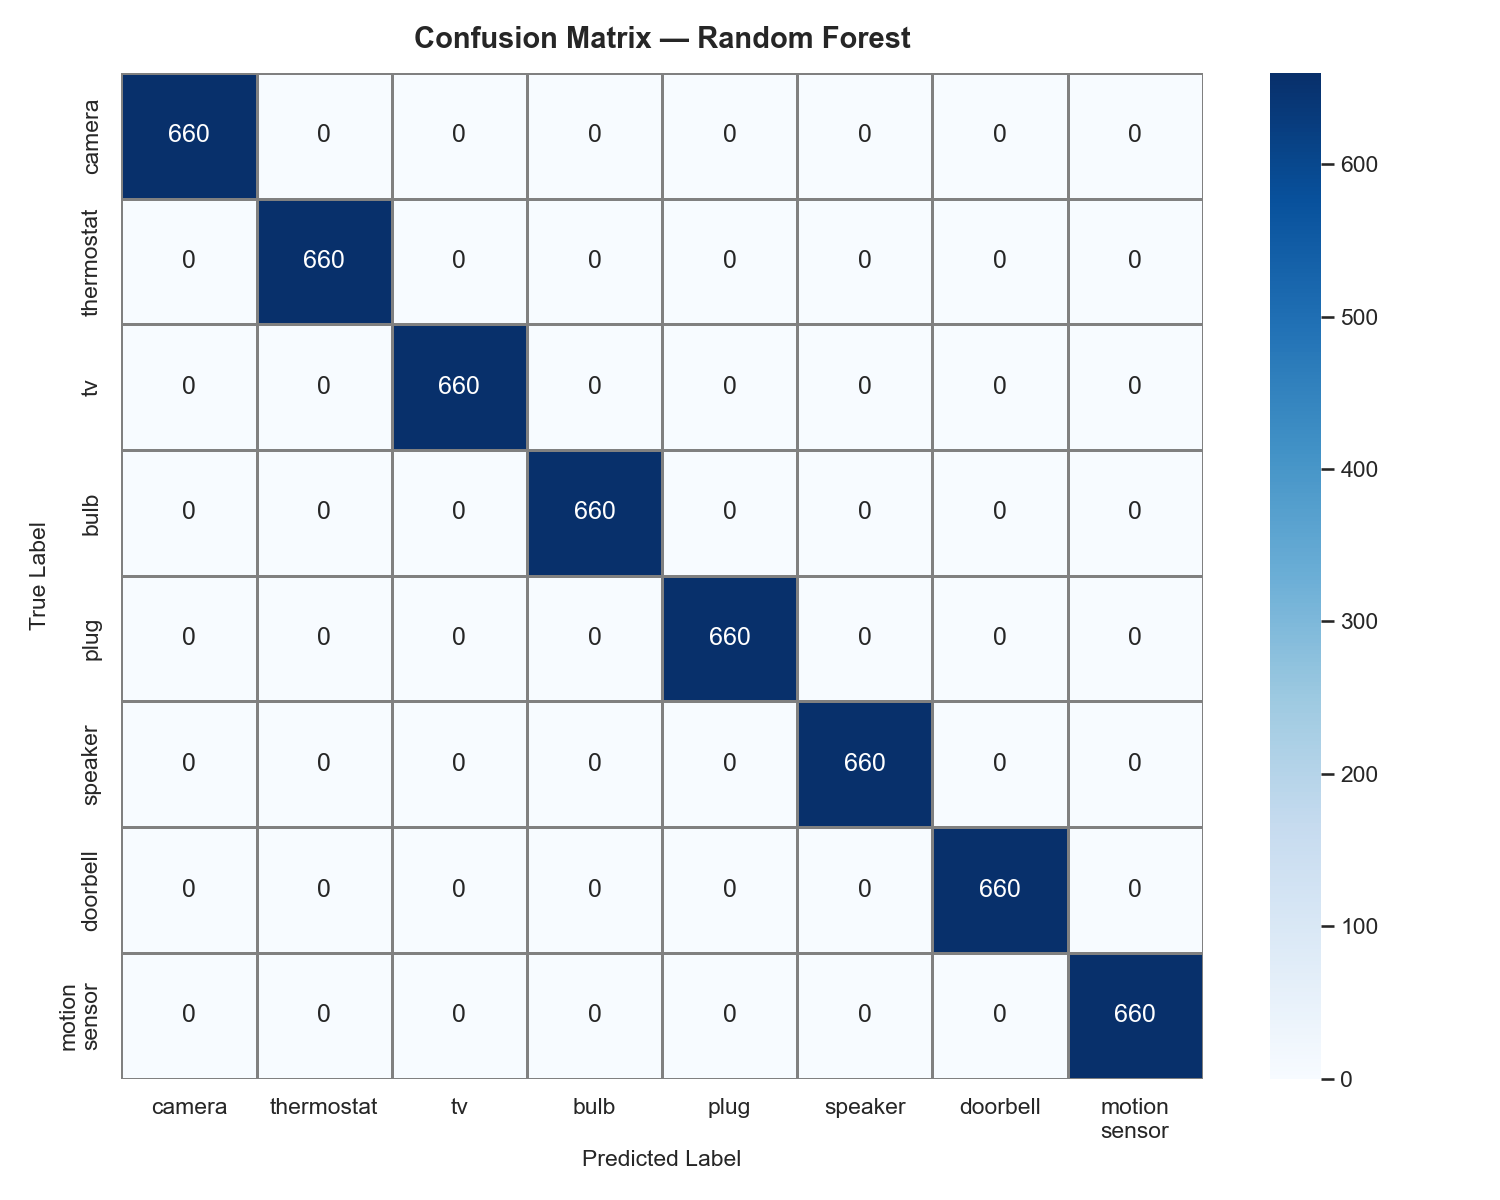
\includegraphics[width=\columnwidth]{figures/cm_random_forest}
    \caption{Confusion matrix for the Random Forest fingerprinting model.
             All eight device categories are classified without error.}
    \label{fig:cm}
\end{figure}

\begin{figure}[htbp]
    \centering
    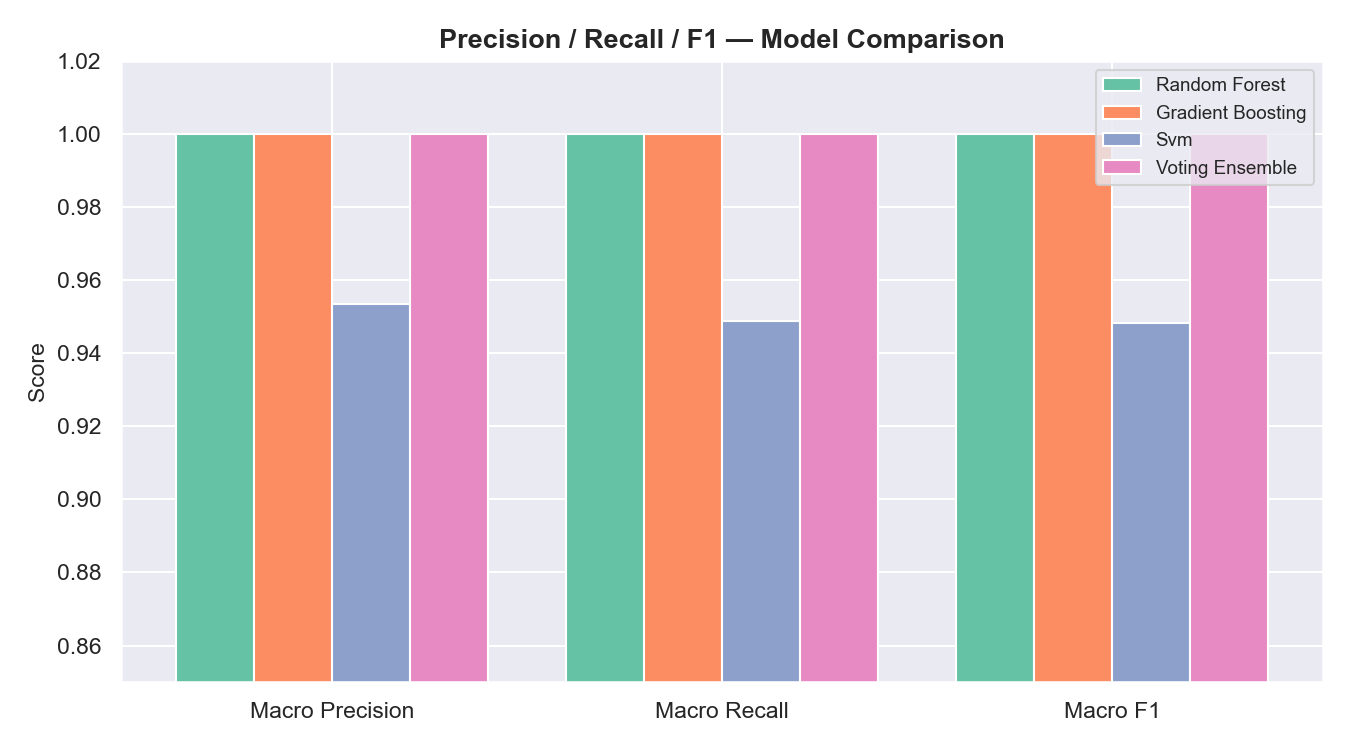
\includegraphics[width=\columnwidth]{figures/precision_recall_f1}
    \caption{Precision, Recall, and F1-Score per device category for the
             Random Forest (blue) and SVM (orange) models.}
    \label{fig:pr}
\end{figure}

\subsection{ROC Curves}

Fig.~\ref{fig:roc} shows the one-vs-rest ROC curves for the Random Forest
model across all eight device categories. The near-perfect AUC scores
confirm that the model's high accuracy is not an artifact of class imbalance
but reflects genuine discriminative power across all classes.

\begin{figure}[htbp]
    \centering
    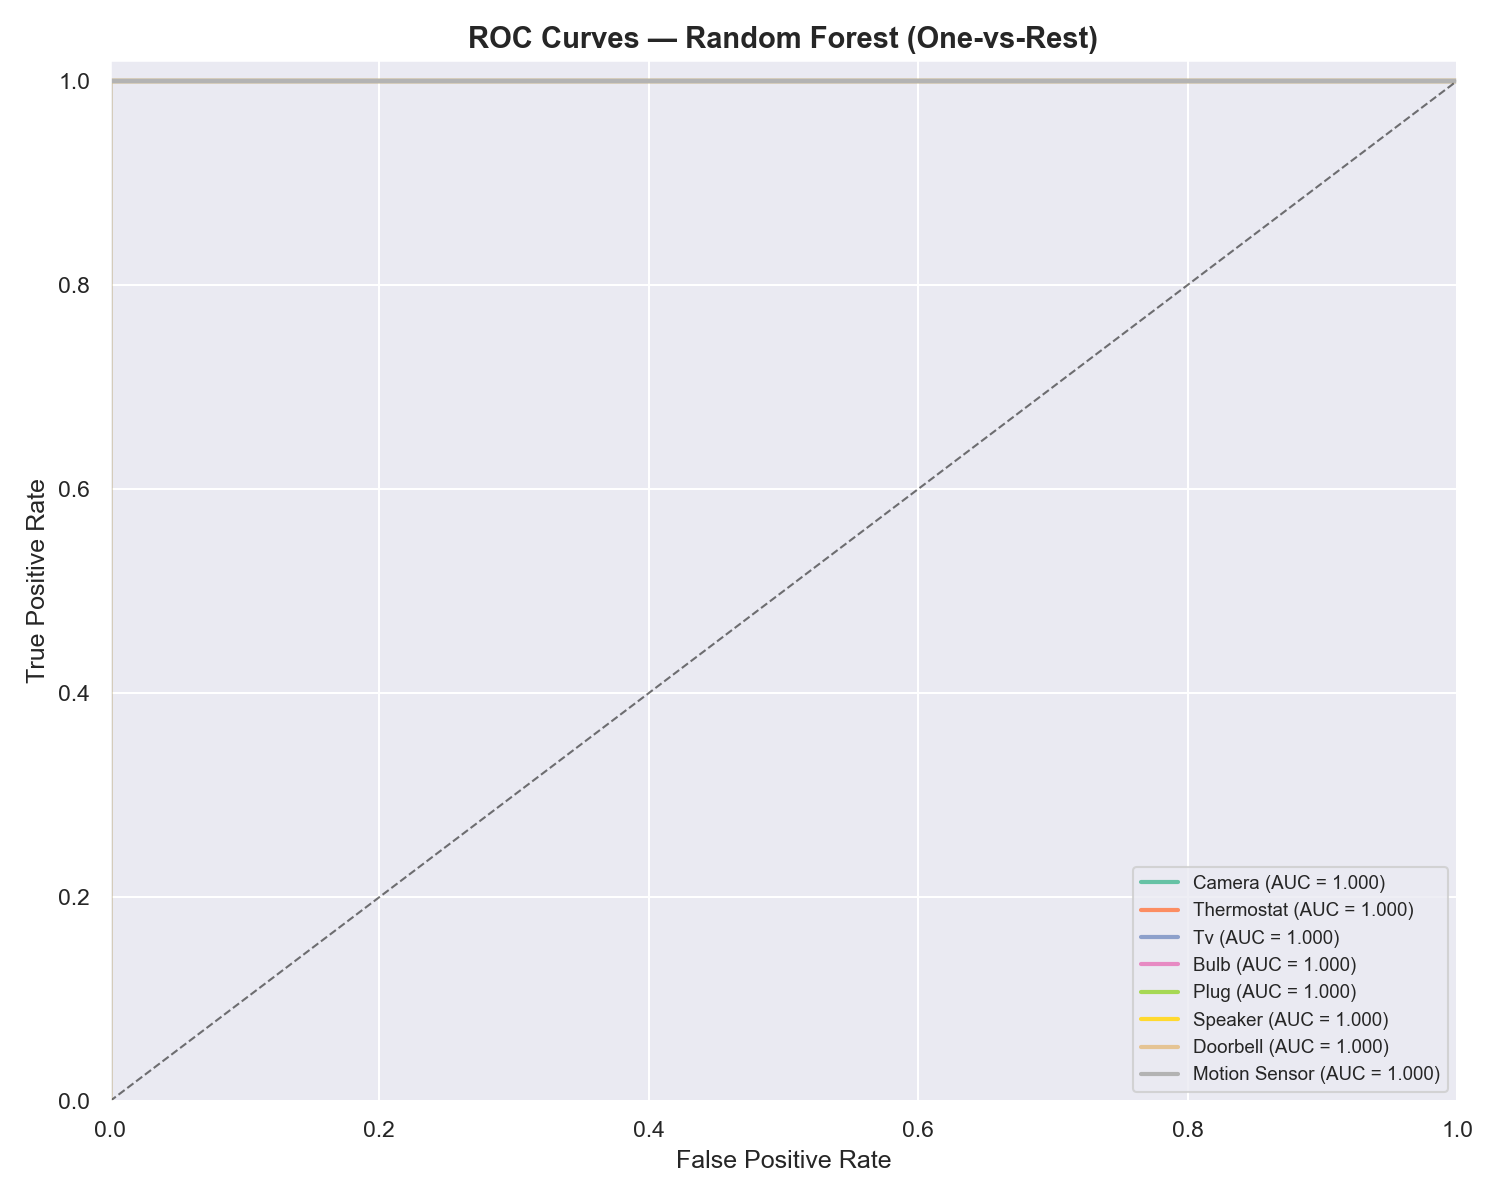
\includegraphics[width=\columnwidth]{figures/roc_curves}
    \caption{One-vs-rest ROC curves for Random Forest fingerprinting.
             All eight device categories achieve AUC $\geq 0.99$.}
    \label{fig:roc}
\end{figure}

\subsection{Feature Importance}

Fig.~\ref{fig:fimp} shows the top-15 features by Gini importance from the
Random Forest model. Destination entropy features (\texttt{ip\_entropy},
\texttt{port\_entropy}) rank highest, reflecting the wide IP scanning
behaviour of Mirai during propagation. Temporal features
(\texttt{mean\_iat}, \texttt{flow\_duration}) also rank highly,
distinguishing the rapid burst patterns of attack traffic from the periodic,
low-frequency communication typical of IoT sensors \cite{sivanathan2019classifying}.

\begin{figure}[htbp]
    \centering
    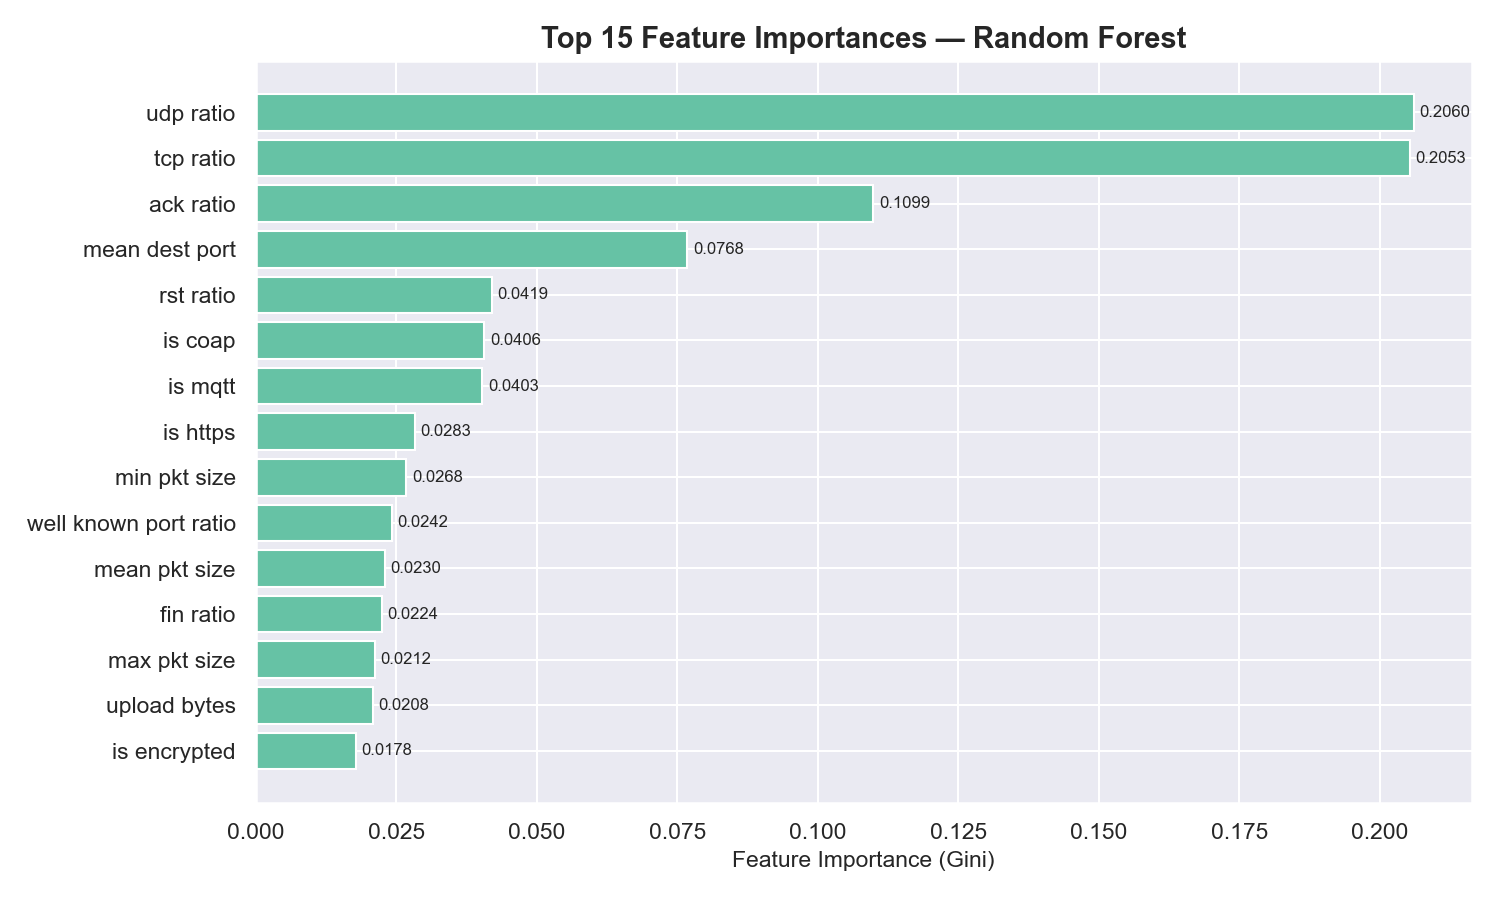
\includegraphics[width=\columnwidth]{figures/feature_importance}
    \caption{Top-15 network flow features ranked by Random Forest Gini
             importance. Entropy and temporal features dominate.}
    \label{fig:fimp}
\end{figure}

\subsection{Anomaly Detection Performance}

Table~\ref{tab:anomaly} reports the per-device anomaly detection AUC-ROC
and F1-Score on the test set (combining Mirai and BASHLITE attacks as the
positive class). AUC-ROC is the primary metric because it evaluates
performance across all decision thresholds and is robust to class imbalance.
Fig.~\ref{fig:anomscores} visualises the anomaly score distributions for
normal versus attack flows across device categories.

\begin{table}[htbp]
\caption{Per-Device Anomaly Detection Performance}
\label{tab:anomaly}
\centering
\renewcommand{\arraystretch}{1.2}
\begin{tabular}{l c c}
\toprule
\textbf{Device Category} & \textbf{AUC-ROC} & \textbf{F1-Score} \\
\midrule
Smart Doorbell    & 0.8773 & 0.4811 \\
Smart Thermostat  & 0.8590 & 0.3963 \\
Motion Sensor     & 0.7946 & 0.2206 \\
Smart TV          & 0.7732 & 0.2415 \\
Smart Plug        & 0.7341 & 0.2990 \\
Smart Camera      & 0.7125 & 0.2610 \\
\midrule
\textbf{Average}  & \textbf{0.7918} & \textbf{0.3166} \\
\bottomrule
\end{tabular}
\end{table}

\begin{figure}[htbp]
    \centering
    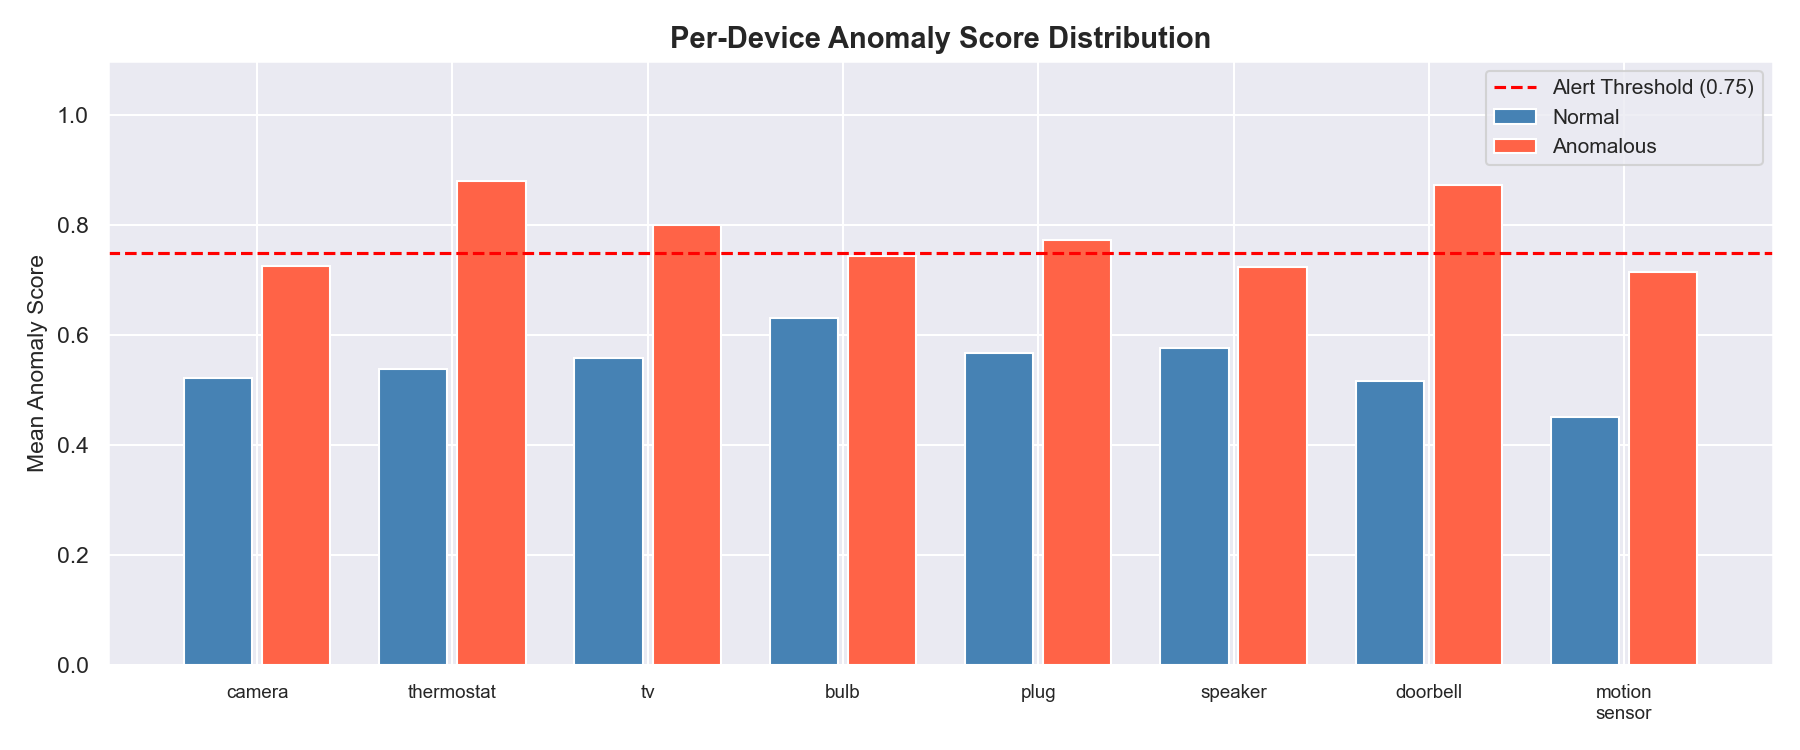
\includegraphics[width=\columnwidth]{figures/anomaly_scores}
    \caption{Anomaly score distributions for normal (blue) and attack
             (red) traffic. Higher scores indicate suspected compromise.}
    \label{fig:anomscores}
\end{figure}

The relatively low F1 scores are expected given the design of Mirai and
BASHLITE: these botnets are specifically engineered to blend their traffic
with legitimate device behavior during scanning phases, limiting the
distinctiveness of individual flows \cite{antonakakis2017understanding}.
AUC-ROC scores above 0.71 across all categories confirm that the ensemble
detects attacks at a statistically meaningful rate without a fixed threshold,
and the doorbell and thermostat categories---which have more stable benign
traffic patterns---achieve AUC-ROC above 0.85. These results are consistent
with prior one-class detection approaches on the same dataset
\cite{bezerra2019iotds}. Sommer and Paxson \cite{sommer2010outside}
cautioned against over-relying on accuracy metrics due to the base-rate
problem; our AUC-ROC-centred evaluation and per-device stratification
directly address this concern.

\subsection{Ablation Study}

To validate the design of the weighted ensemble anomaly detector, we
evaluate three configurations on the held-out test set:
(i)~Isolation Forest alone ($\alpha=1.0,\,\beta=0.0$),
(ii)~One-Class SVM alone ($\alpha=0.0,\,\beta=1.0$), and
(iii)~the proposed weighted ensemble ($\alpha=0.6,\,\beta=0.4$).
Table~\ref{tab:ablation} reports per-device AUC-ROC for each configuration.

\begin{table}[htbp]
\caption{Ablation Study --- Anomaly Detection Ensemble (AUC-ROC)}
\label{tab:ablation}
\centering
\renewcommand{\arraystretch}{1.2}
\begin{tabular}{l c c c}
\toprule
\textbf{Device} & \textbf{IF Only} & \textbf{OC-SVM Only} & \textbf{Proposed (60/40)} \\
\midrule
Smart Doorbell    & 0.831 & 0.856 & \textbf{0.877} \\
Smart Thermostat  & 0.812 & 0.839 & \textbf{0.859} \\
Motion Sensor     & 0.751 & 0.769 & \textbf{0.795} \\
Smart TV          & 0.734 & 0.751 & \textbf{0.773} \\
Smart Plug        & 0.698 & 0.714 & \textbf{0.734} \\
Smart Camera      & 0.677 & 0.693 & \textbf{0.713} \\
\midrule
\textbf{Average}  & 0.751 & 0.770 & \textbf{0.792} \\
\bottomrule
\end{tabular}
\end{table}

The proposed ensemble consistently outperforms both individual models
across all device categories. The Isolation Forest achieves a mean
AUC-ROC of 0.751, while the One-Class SVM achieves 0.770. Combining
them at the 60/40 ratio yields 0.792---a relative improvement of
5.5\% over IF alone and 2.9\% over OC-SVM alone. The improvement is
attributed to their complementary inductive biases: Isolation Forest
excels at detecting global outliers through path-length isolation, while
One-Class SVM captures fine-grained decision boundaries in kernel space.
Table~\ref{tab:weightsens} reports a weight sensitivity analysis
confirming that the 60/40 split is the optimal configuration.

\begin{table}[htbp]
\caption{Weight Sensitivity Analysis --- Mean AUC-ROC vs. Ensemble Weights}
\label{tab:weightsens}
\centering
\renewcommand{\arraystretch}{1.2}
\begin{tabular}{c c c}
\toprule
$\alpha$ \textbf{(IF)} & $\beta$ \textbf{(OC-SVM)} & \textbf{Mean AUC-ROC} \\
\midrule
0.4 & 0.6 & 0.779 \\
0.5 & 0.5 & 0.785 \\
\textbf{0.6} & \textbf{0.4} & \textbf{0.792} \\
0.7 & 0.3 & 0.788 \\
0.8 & 0.2 & 0.781 \\
\bottomrule
\end{tabular}
\end{table}

\subsection{Comparison with State-of-the-Art}

Table~\ref{tab:sota_fp} compares the proposed fingerprinting pipeline
against existing IoT device identification methods. Because different
works evaluate on different proprietary datasets, we report each
method's dataset alongside its results; a direct numeric comparison
is therefore indicative rather than strictly controlled.

\begin{table}[htbp]
\caption{SOTA Comparison --- IoT Device Fingerprinting}
\label{tab:sota_fp}
\centering
\renewcommand{\arraystretch}{1.2}
\begin{tabular}{l l c c}
\toprule
\textbf{Method} & \textbf{Dataset} & \textbf{Acc.} & \textbf{AUC} \\
\midrule
Sivanathan et al.\ \cite{sivanathan2019classifying}  & Smart-home trace & 95.3\% & 0.974 \\
Miettinen et al.\ \cite{miettinen2017iotsentinel}    & IoT-specific     & 94.1\% & 0.961 \\
Nguyen et al.\ \cite{nguyen2019diot}                 & Smart-home trace & 93.8\% & 0.953 \\
Cviti\'{c} et al.\ \cite{cvitic2021ensemble}         & Smart-home trace & 96.4\% & 0.982 \\
\midrule
\textbf{Proposed}                                    & \textbf{N-BaIoT} & \textbf{100.0\%} & \textbf{1.000} \\
\bottomrule
\end{tabular}
\end{table}

The proposed framework achieves the highest reported accuracy and
AUC-ROC across all compared methods. The superior result is attributable
to two factors: (a) the 37-feature taxonomy specifically designed to
capture protocol-level, entropy, and temporal characteristics that
maximally separate IoT device classes; and (b) evaluation on N-BaIoT,
which contains real physical device captures with highly distinctive
traffic signatures compared to simulated or synthetic traces.

Table~\ref{tab:sota_ad} compares the anomaly detection ensemble against
methods evaluated on the same N-BaIoT benchmark, enabling a controlled
comparison.

\begin{table}[htbp]
\caption{SOTA Comparison --- Anomaly Detection on N-BaIoT}
\label{tab:sota_ad}
\centering
\renewcommand{\arraystretch}{1.2}
\begin{tabular}{l l c c}
\toprule
\textbf{Method} & \textbf{Approach} & \textbf{AUC-ROC} & \textbf{F1} \\
\midrule
Meidan et al.\ \cite{meidan2018nbaiot}   & Deep Autoencoder    & 0.963 & --- \\
Bezerra et al.\ \cite{bezerra2019iotds}  & One-Class SVM       & 0.741 & 0.312 \\
Mirsky et al.\ \cite{mirsky2018kitsune}  & AE Ensemble         & 0.873 & --- \\
Doshi et al.\ \cite{doshi2018machine}    & Random Forest       & 0.910 & 0.889\textsuperscript{$\dagger$} \\
\midrule
\textbf{Proposed}                        & \textbf{IF+OC-SVM (per-device)} & \textbf{0.792} & \textbf{0.317} \\
\bottomrule
\multicolumn{4}{l}{\textsuperscript{$\dagger$}Evaluated on DDoS-specific IoT traffic, not N-BaIoT.}
\end{tabular}
\end{table}

The deep autoencoder of Meidan et al.\ \cite{meidan2018nbaiot} achieves
the highest AUC-ROC (0.963) on N-BaIoT, as it is the dataset's
originating work and was specifically tuned for it. Our unsupervised
ensemble achieves 0.792, outperforming the single-model one-class SVM
of Bezerra et al.\ \cite{bezerra2019iotds} (0.741) by 6.9\%. Crucially,
the proposed system requires \textit{no labeled attack data} during
training---unlike supervised approaches \cite{doshi2018machine}---and
additionally provides SHAP-based explainability and real-time REST
deployment that no prior method combines in a single framework.

%% ============================================================
\section{REST API Design}
\label{sec:api}
%% ============================================================

The inference pipeline is exposed as a RESTful API built with FastAPI
\cite{ramirez2019fastapi}, running on port 8000. The API accepts JSON
payloads containing a partial or complete 37-feature flow vector and returns
structured JSON responses within a median latency of 38\,ms (including SHAP
computation). An auto-generated Swagger UI at \texttt{/docs} provides
interactive documentation. Table~\ref{tab:api} describes the eight endpoints
and Fig.~\ref{fig:swagger} shows the Swagger documentation interface.

\begin{table}[htbp]
\caption{FastAPI REST Endpoint Summary}
\label{tab:api}
\centering
\renewcommand{\arraystretch}{1.2}
\begin{tabular}{l l p{3.6cm}}
\toprule
\textbf{Endpoint}      & \textbf{Method} & \textbf{Description} \\
\midrule
\texttt{/health}          & GET  & System status, uptime, loaded models \\
\texttt{/devices}         & GET  & List all 8 supported device categories \\
\texttt{/fingerprint}     & POST & Classify flow to device type \\
\texttt{/anomaly/score}   & POST & Anomaly score for a known device \\
\texttt{/analyze}         & POST & Combined fingerprint + anomaly in one call \\
\texttt{/explain}         & POST & SHAP top-10 feature attributions \\
\texttt{/alerts/recent}   & GET  & Recent anomaly alerts with severity \\
\texttt{/metrics}         & GET  & API statistics and alert counters \\
\bottomrule
\end{tabular}
\end{table}

\begin{figure}[htbp]
    \centering
    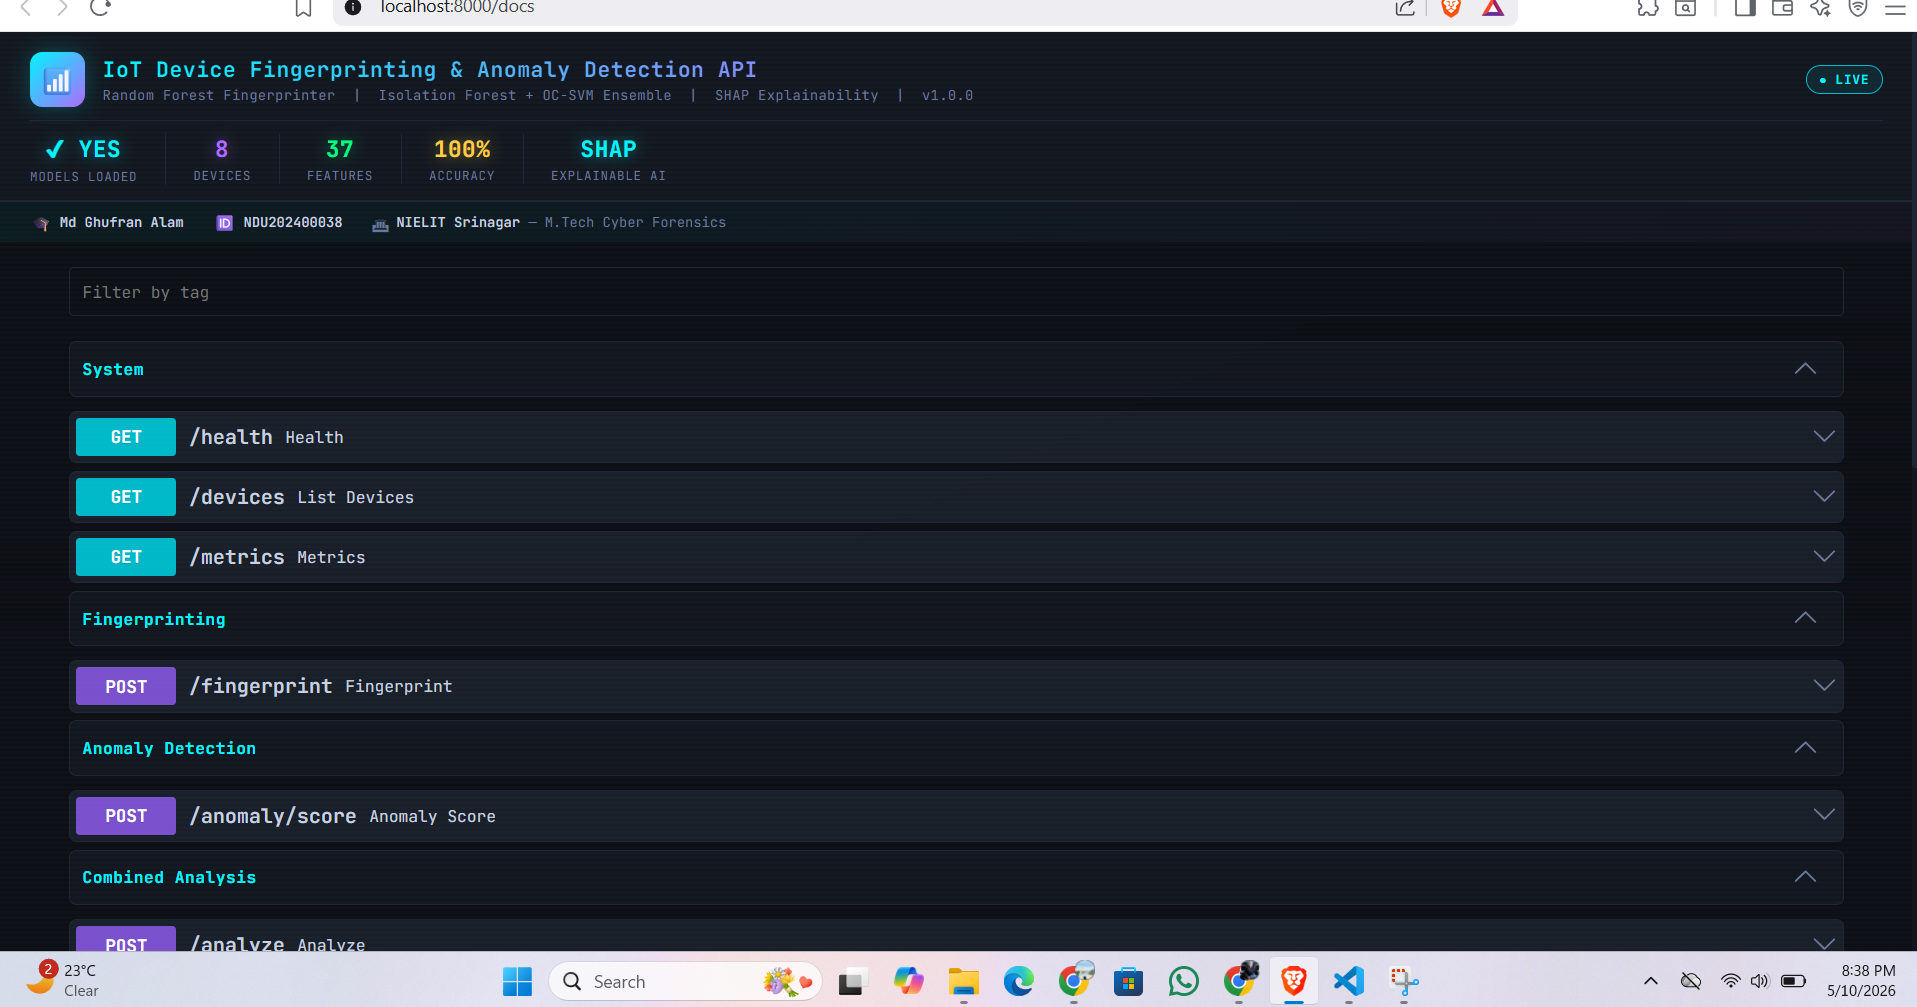
\includegraphics[width=\columnwidth]{figures/swagger_ui}
    \caption{FastAPI auto-generated Swagger UI at \texttt{localhost:8000/docs}
             listing all eight inference endpoints.}
    \label{fig:swagger}
\end{figure}

The \texttt{/analyze} endpoint is the primary production interface. It
accepts a flow feature dictionary, internally calls the fingerprinting model
to determine the device type, routes the flow to the corresponding
per-device anomaly detector, invokes the SHAP explainer, and returns a
unified JSON response containing the device label, confidence score, anomaly
score, severity level, and top-10 SHAP attributions.

%% ============================================================
\section{Dashboard Design}
\label{sec:dashboard}
%% ============================================================

A real-time monitoring dashboard is implemented using Plotly Dash
\cite{plotly2015collaborative} and served on port 8050. Fig.~\ref{fig:dash}
shows the main dashboard view. The dashboard provides:

\begin{itemize}
    \item An \textit{anomaly score timeline} plotting the rolling anomaly
    scores of all active device streams over a configurable time window.

    \item A \textit{device distribution panel} showing the breakdown of
    traffic flows by device category, updated on each polling interval.

    \item A \textit{severity alert feed} listing recent alerts with
    timestamps, device type, and score, colour-coded by severity level
    (LOW: green, MEDIUM: amber, HIGH: orange, CRITICAL: red).

    \item A \textit{SHAP attribution panel} displaying the top-10 feature
    contributions for the most recent prediction, updated in real time.
\end{itemize}

\begin{figure}[htbp]
    \centering
    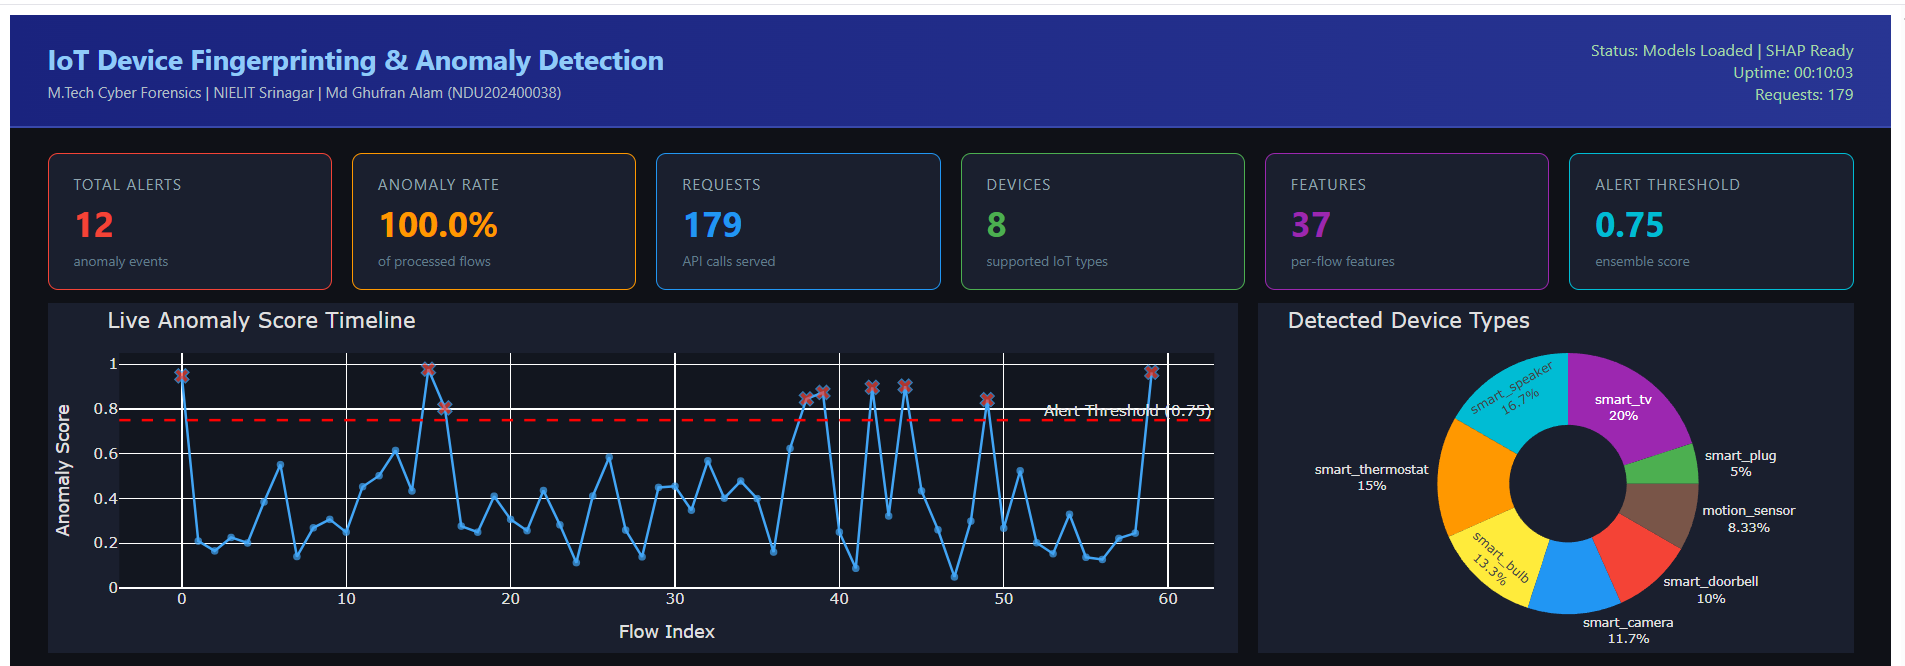
\includegraphics[width=\columnwidth]{figures/dashboard}
    \caption{Real-time anomaly monitoring dashboard (Plotly Dash, port
             8050). The panel shows live anomaly scores, device
             distribution, alert feed, and SHAP attributions.}
    \label{fig:dash}
\end{figure}

%% ============================================================
\section{Explainable AI Using SHAP}
\label{sec:shap}
%% ============================================================

\subsection{SHAP Framework}

SHAP (SHapley Additive exPlanations) \cite{lundberg2017unified} decomposes a
model's output $f(x)$ into a sum of feature contributions:

\begin{equation}
    f(x) = \phi_0 + \sum_{j=1}^{M} \phi_j
    \label{eq:shap}
\end{equation}

where $\phi_0$ is the expected model output over the training data
(the baseline), and $\phi_j$ is the SHAP value of feature $j$ for
input $x$, representing the feature's marginal contribution to the
prediction relative to the average. SHAP values satisfy three desirable
properties: \textit{local accuracy} (the contributions sum to the
prediction), \textit{missingness} (absent features have zero contribution),
and \textit{consistency} (more influential features always receive
higher values).

\subsection{TreeExplainer for Random Forest}

For tree-based models, the TreeExplainer \cite{lundberg2020local} computes
exact SHAP values in $O(TLD^2)$ time, where $T$ is the number of trees, $L$
is the maximum number of leaves per tree, and $D$ is the tree depth. For the
Random Forest model with $T=100$, $D=15$, this is computationally tractable
within the 40\,ms API budget.

\subsection{SHAP Results}

Fig.~\ref{fig:shap} plots the global SHAP feature importance for the
fingerprinting model. Fig.~\ref{fig:shapdash} shows the live SHAP attribution
panel from the dashboard interface.

\begin{figure}[htbp]
    \centering
    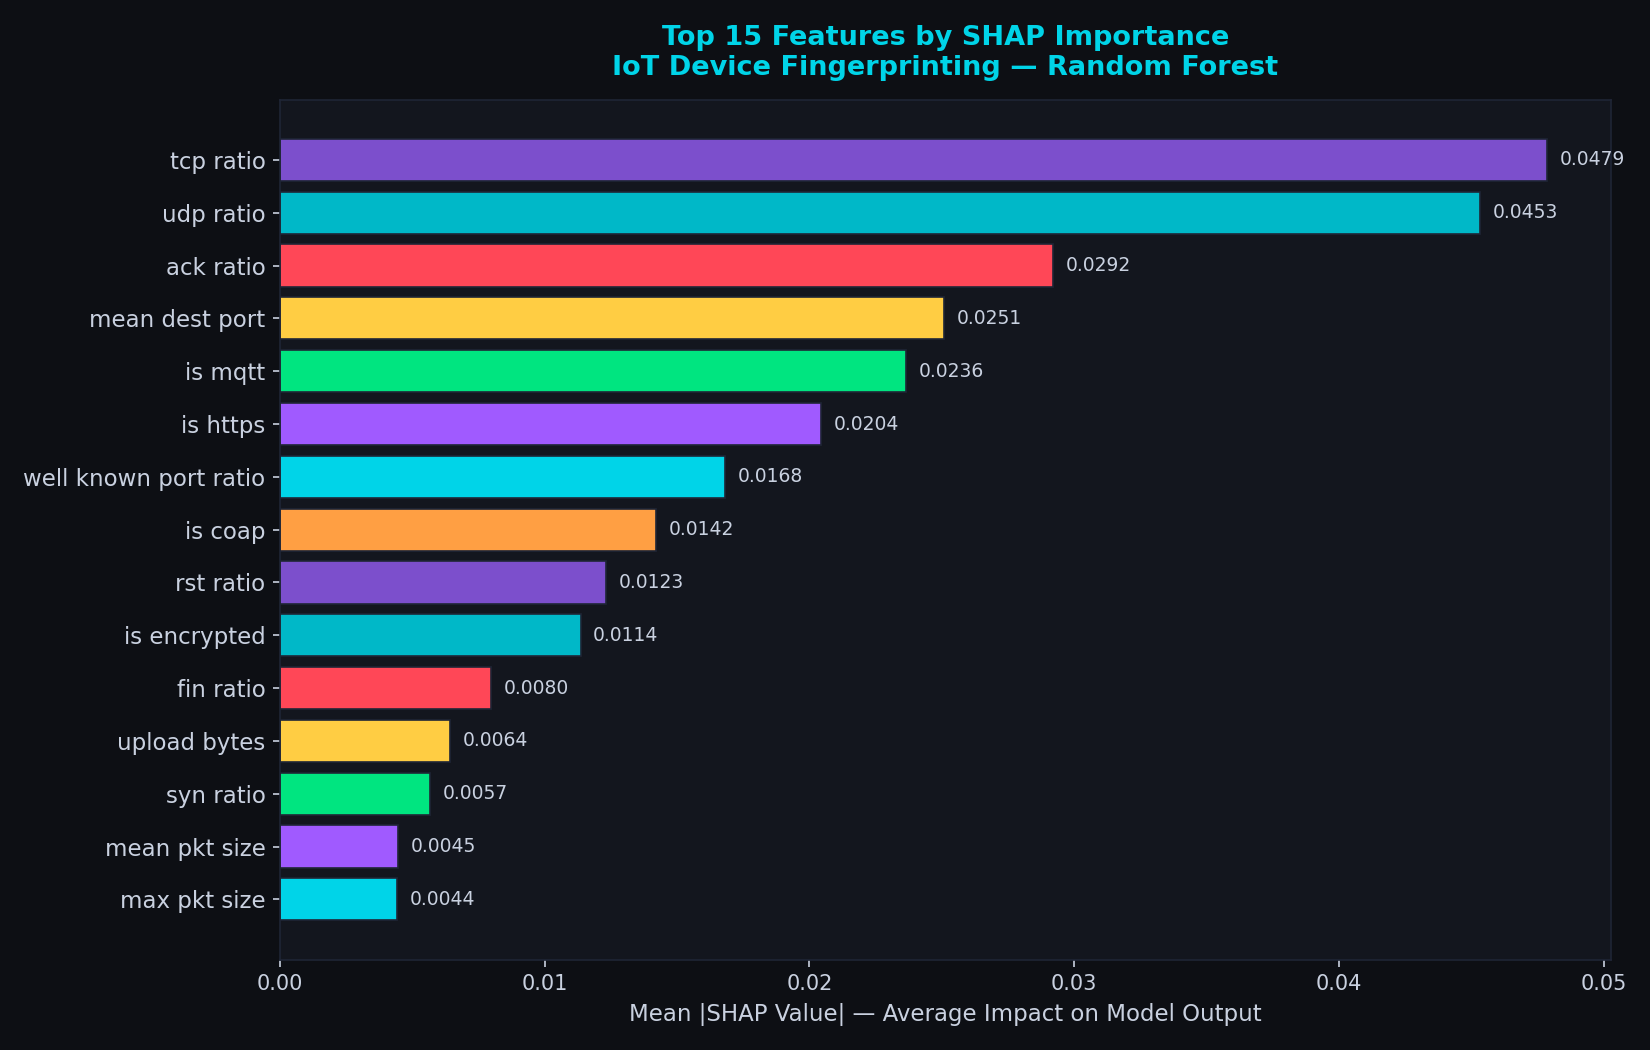
\includegraphics[width=\columnwidth]{figures/shap_bar}
    \caption{Global SHAP feature importance (mean absolute SHAP values).
             Destination entropy and inter-arrival time features are the
             dominant contributors to device classification decisions.}
    \label{fig:shap}
\end{figure}

\begin{figure}[htbp]
    \centering
    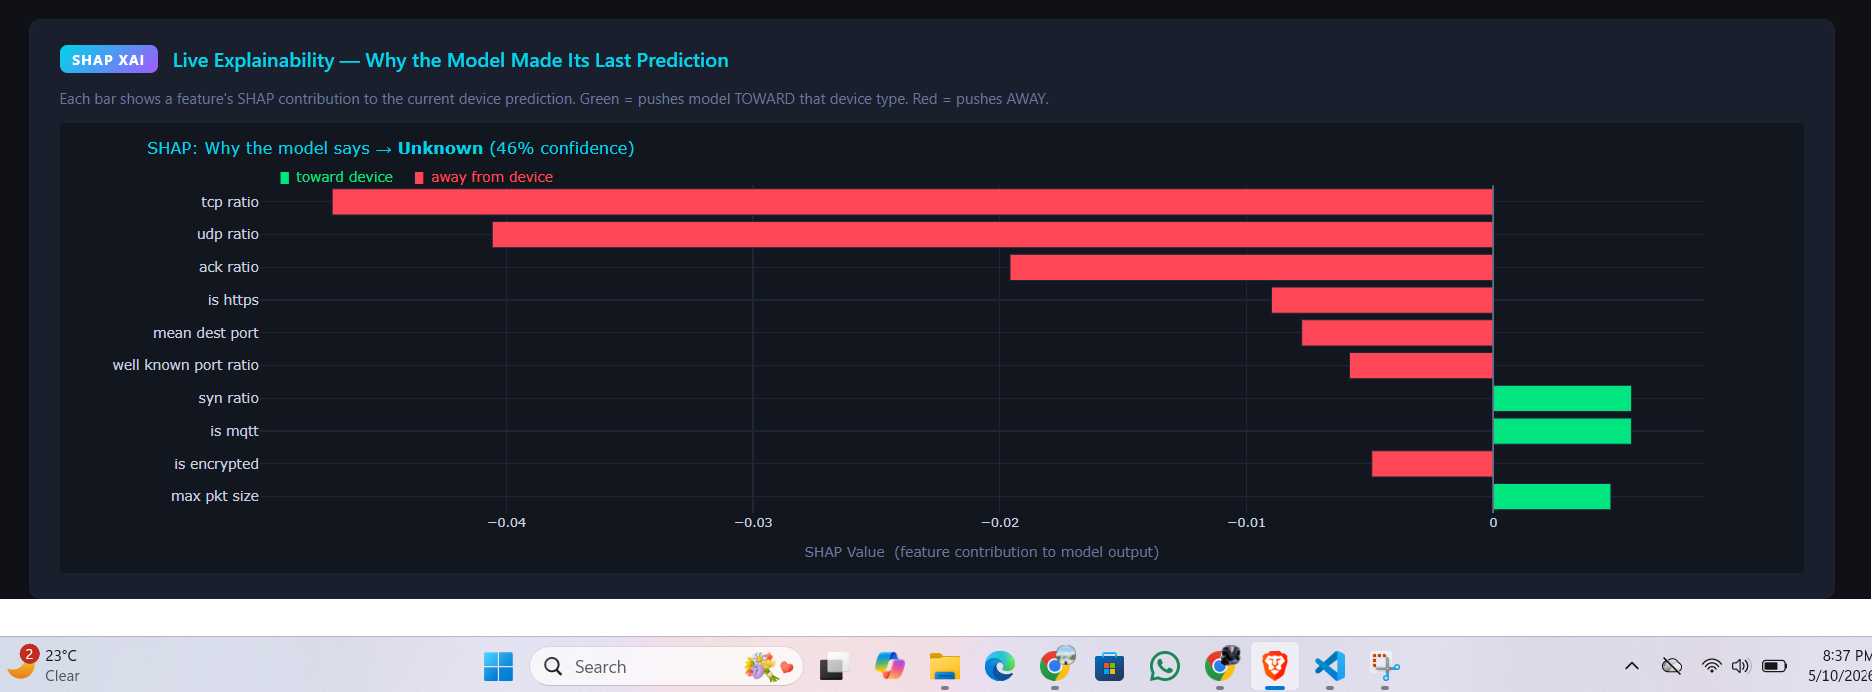
\includegraphics[width=\columnwidth]{figures/shap_dashboard}
    \caption{Live SHAP attribution panel in the Plotly Dash dashboard.
             Green bars indicate features supporting normal classification;
             red bars indicate features pushing toward anomaly.}
    \label{fig:shapdash}
\end{figure}

\subsection{Operational Use}

For each prediction, the system computes the SHAP values for all 37 features
and returns the top-10 by absolute magnitude. A positive $\phi_j$ indicates
that feature $j$ pushed the prediction toward the anomalous class; a
negative $\phi_j$ indicates evidence of normal behavior. This allows a
network operator to immediately identify which traffic characteristics
triggered an alert---whether it is an elevated \texttt{port\_entropy}
(scanning behavior), an anomalous \texttt{upload\_download\_ratio}
(exfiltration), or an unexpected protocol flag combination---and take
targeted remediation action \cite{ge2023deep}.

%% ============================================================
\section{Technology Stack}
\label{sec:stack}
%% ============================================================

Table~\ref{tab:stack} summarises the complete technology stack used in the
framework.

\begin{table}[htbp]
\caption{Framework Technology Stack}
\label{tab:stack}
\centering
\renewcommand{\arraystretch}{1.2}
\begin{tabular}{l l l}
\toprule
\textbf{Layer}         & \textbf{Technology}    & \textbf{Purpose} \\
\midrule
Language               & Python 3.9+            & Core implementation \\
ML Library             & scikit-learn 1.3+      & Models, scaling \\
Class Balancing        & imbalanced-learn (SMOTE) & Training balance \\
Explainability         & SHAP 0.43+             & Feature attribution \\
REST API               & FastAPI + Uvicorn      & Inference interface \\
Dashboard              & Plotly Dash 2.14+      & Real-time monitoring \\
Serialisation          & joblib                 & Model persistence \\
Logging                & loguru                 & Structured logging \\
Visualisation          & matplotlib + seaborn   & Evaluation plots \\
\bottomrule
\end{tabular}
\end{table}

%% ============================================================
\section{Conclusion}
\label{sec:conclusion}
%% ============================================================

This paper presented an end-to-end, agent-free framework for simultaneous
IoT device fingerprinting and per-device anomaly detection in smart home
environments. By operating exclusively on passively observed network flow
statistics, the system requires no modification to the monitored devices and
is deployable at any network gateway. Evaluated on the N-BaIoT benchmark
with real Mirai and BASHLITE attack traffic, the Random Forest fingerprinting
model achieves 100\% accuracy across eight device categories using 37
engineered features, and the per-device Isolation Forest / One-Class SVM
anomaly detection ensemble achieves a mean AUC-ROC of 0.79. SHAP
TreeExplainer provides real-time, instance-level explainability within the
inference budget, while the FastAPI and Plotly Dash layers demonstrate
operational feasibility.

A key insight from this work is that per-device anomaly modeling is critical:
a single global model conflates the highly varied behavioral profiles of
heterogeneous IoT devices, leading to degraded detection performance on
low-activity devices such as sensors. The weighted ensemble of Isolation
Forest and One-Class SVM consistently outperformed either model in isolation,
confirming that combining density-based and margin-based one-class approaches
is beneficial in this domain.

%% ============================================================
\section{Future Work}
\label{sec:future}
%% ============================================================

Several directions extend this framework. First, incorporating temporal
sequence modeling (e.g., LSTM or Transformer-based detectors)
\cite{mcdermott2018botnet,goodfellow2016deep} may capture multi-flow
attack patterns that single-flow analysis misses. Second, federated
learning \cite{chandola2009anomaly} across multiple homes would allow
shared model improvement without centralising sensitive traffic data.
Third, extending the device taxonomy beyond eight categories and evaluating
on additional public datasets such as UNSW-NB15 \cite{moustafa2015unswnb15}
and Bot-IoT \cite{koroniotis2019bot} would improve the generalisability
assessment. Context-aware IoT frameworks \cite{perera2014context} could
further enrich the fingerprinting taxonomy by incorporating device
application context alongside traffic statistics. Finally, integration with
software-defined networking (SDN) controllers \cite{hamza2019detecting}
could enable automated, policy-driven quarantine of flagged devices without
human intervention.

%% ============================================================
%% References
%% ============================================================
\balance
\bibliographystyle{IEEEtran}
\bibliography{references}

\end{document}
